\section{Introduction}
\label{sec:intro}
In Chapter \ref{ch:mapping}, we presented our approach for automatic transformation of business process models into Reo~\cite{behnaz}. This enables the use of Reo analysis methods and tools on these processes that originally were not expressed in Reo.
Performing analysis on a Reo connector requires the behavior of the connector expressed in one of the formal semantics of Reo. 

Each of these formal semantics comes with a set of definitions and operators, which enable calculating semantics of a Reo connector. The straight-forward algorithms of supporting tools for automating this process are developed based on these definitions. These custom algorithms are computationally expensive and not optimized. As a result, in practice the size of a connector they can support is small.  

Another inherent limitation of these algorithms stem from that they model data explicitly. As a consequence, in practice the set of input data needs to be limited to a predefined small set. This holds even for connecters with no data-sensitive components, which shows the same behavior for each data item.

Even though different formal semantics of a Reo connector describe the behavior of the same model, since each of them focuses on some behavioral aspects such as context-sensitivity or data-awareness, and ignores some other aspects, it is possible that one aspects of its semantics describes some behavior that another semantics considers invalid. 
A classical example of this case is when a \emph{lossySync} channel is connected to a \emph{FIFO}$_1$ channel. The constraint automata and the coloring semantics for this example describe different behavior. 

In this chapter, we present a constraint-based framework to derive formal semantics of a Reo connector. We form a constraint by encoding the behavior of constructs of the connector. 

Our framework eliminates the result of expressiveness gap among Reo formal semantics by incorporating more than one semantics in deriving the behavior of a Reo connector. 
This way, we transform problem of calculating formal semantics of a Reo connector into a constraint satisfaction problem, for which efficient and optimized methods and tools exist. We use the symbolic approach to deal with data, i.e, rather than dealing with concrete values, we split the data domain to ranges for which the connector exhibits different behavior. 

This work is a necessary step for providing fully automated model checking for data-aware and context-dependent Reo connectors. It can be seen as a generalization of the constraint-based framework presented in \cite{JoseThesis}, that is used as a base for Reo's distributed execution engine. However, there are major differences between them. For instance, the framework for the Reo execution engine only provide support for synchrony and context-sensitivity, while our method deals with priority and data-constraints as well.

%
%Service-oriented architecture~\cite{soabell2008introduction} (SOA) is a relatively recent trend in software development. The SOA implementation depends on a mesh of functionality units, called services. Services are loosely coupled and do not invoke or communicate with each other directly. Instead, they employ a pre-defined protocol, which specifies the way they can exchange messages amongst themselves. As a result, the correctness of a SOA implementation relies not only on the correctness of its involved services but also on the properness of its communication protocol.
%
%Coordination languages and models provide dedicated frameworks to study the communication protocols as separate concerns. They define the ``glue code'' that ties together the services to enable the message passing among the involved services. Some recent coordination models include: i) a Calculus for Orchestration of Web Services (COWS) \cite{cowsPuglieseT12}, which specifies the combination of service-oriented applications and models their dynamic behavior; ii) Orc \cite{orc06}, a process calculus for distributed and concurrent programming which provides uniform access to computational services, including distributed communication and data manipulation; and  iii) Reo~\cite{Arbab04RCC}, an exogenous coordination language that realizes the coordination patterns in terms of its complex \emph{connector}s, also called \emph{network}s, that are built out of simple primitives called \emph{channel}s. In the sequel, we focus on Reo.
%
%~\cite{bpmn}
%Each channel in Reo defines a form of coordination in terms of synchronizing, buffering, retaining data, etc., along with constraining its input and output data items. Reo allows hierarchical modeling where arbitrarily complex connectors can be formed out of simpler networks. The suitability of Reo to model behavioral patterns describable by business process models has been already studied \cite{bpmn2reo} \cite{behnaz}. We have also developed tools for automatic transformation of these models into Reo~\cite{behnaz}. This enables the use of Reo analysis methods and tools on the coordination protocols that originally were not expressed in Reo. 
%ing Notation (BPMN),  Business Process Execution Language (BPEL)~\cite{bpel} and the most common Unified Modeling Language (UML) 2.0~\cite{uml} dynamic models: Activity diagrams and Sequence diagrams. We have also developed tools for automatic transformation of these models into Reo~\cite{behnaz}. This enables the use of Reo analysis methods and tools on the coordination protocols that originally were not expressed in Reo. 
%Several extensions for CA have been proposed, among them, Constraint Automata with State Memory (CASM)~\cite{CASMPourvatan2009}, Action Constraint Automata (ACA) \cite{kokash2010semantic}, and Quantitative Intensional Automata (QIA)~\cite{qia}. Each of these semantics focuses on certain aspects of Reo and is used in the areas that need its special expressiveness. The Extensible Coordination Tool-set (ECT)~\cite{ect} is a framework that integrates several tools to analyze Reo networks. Among them is the Reo animation engine~\cite{ect}, which allows a visual validation of the protocol by generating animated simulation of the connector. Although animation is useful for giving insight about the behavior of networks, due to its manual nature and lack of support for data-dependent behavior, its application is limited to special cases. 
%The automatic analysis tools integrated in ECT include the model checker Vereofy~\cite{vereofy}, the converter and model checker based on mCRL2~\cite{natmcrl2jor} and the stochastic analyzer tool integrated with Prism~\cite{prismyoungjoo}. Related to the field of our interest, formal testing and test generation, Aichering et al.~\cite{aichernig2009fault} implemented a testing tool for Reo based on the rewriting logic Maude. They remark that since in Reo not every input event leads to an output, testing theories for finite state machines do not suit for testing Reo. In our previous work~\cite{kokash2011input}, we have employed the input-output conformance (ioco) testing theory for model-based testing and test generation for coordination  protocols modeled in Reo. There, we use the automata based underlying semantics of Reo to translate connectors to their equivalent process algebra, from which we  generate their corresponding input-output labeled transitions systems to feed to the TorX~\cite{torx}testing 
%
% A shortcoming of earlier work stems from its lack of support for data-dependent behavior. We overcome this shortcoming in the work we present in this thesis. Our tool is a necessary step for providing fully automated model checking for data-aware and context-dependent composition of services coordinated by Reo.
%Similar to most formal verification approaches, a major problem while working with ECT is the state explosion. %The freedom that Reo provide in having multiple concurrent data-flows is one of the origin of the  along with the data domain non-determinism in behavior of some channels are some origins of the bug state space.
 %Avoiding the state space explosion is crucial while dealing with data-dependent channels especially if we are interested in working with infinite data-domains. A traditional remedy for this problem is abstraction. In this paper, we show how using computer algebra systems, namely Reduce~\cite{reduce}, can improve the situation. 
 % Our approach is to partition the data-domain into regions for which a model reacts differently and represent each region as a single data-item. Since the number of data sensitive elements in each Reo model is finite, this solution guarantees the finiteness  of the abstract data domain. Based on this approach, we have implemented a plug-in for ECT that generates ioco test for a given Reo network. 
%Reducing the range of data to 
 %?The high degree of concurrency in Reo models makes a big state st  Another problem that a user face while working with the current Reo based tool-set is 

%The rest of this chapter is organized as follows. In Section 2, we explain the basics of Reo. In Section 3, we introduce constraint automata with state memory. In Section 4, we formalize the mentioned semantic model of Reo in systems of constraints along with techniques to solve them. In Section 5, we show how we abstract from the internal ports in a Reo network in a minimized representation. In Section 6, we briefly discuss some properties of our presented constraint encoding of Reo networks. Finally, in Section 7, we conclude the chapter and outline our future work.

\section{Reo constraint satisfaction problem (RCSP)}
\label{sec:ecsp}
%In Section \ref{ssec:formalsem}, we presented an overview of the various behavioral dimensions of a Reo network. 
In this section, we extend the constraint-based framework in \cite{JoseThesis} to incorporate all behavioral dimensions addressed by various semantic models for Reo. In our framework, we denote each of these elements by variables over their proper domains. 

We relate these variables to each other and restrict possible values they can assume using constraints whose solutions give the underlying formal semantics of the network. In this section, we deal only with connectors whose semantics can be expressed in CASM or CC. Later, we extend our framework to also support priority.

Let $\mathcal{N} = \mathcal{N}^{src} \cup \mathcal{N}^{mix} \cup \mathcal{N}^{snk}$ be the global set of nodes, $\mathcal{M}$ the global set of state memory variables, and $\mathcal{D}$ the global set of numerical data values. The set of primitive ends $\mathcal{P}$ consists of all primitive ends $p$ derived from $\mathcal{N}$ by marking its elements with superscripts $c$ and $k$, according to the following grammar:
$$
p ::= r^c ~|~ s^k 
$$

\noindent
where $r \in \mathcal{N}^{src} \cup \mathcal{N}^{mix}$ and $s \in \mathcal{N}^{snk} \cup \mathcal{N}^{mix}$. Observe that the primitive ends $n^c$ and $n^k$ connect on the common node $n$.

Let $p \in \mathcal{P}$, $n \in \mathcal{N}$ and $m \in \mathcal{M}$ be a primitive end, a node, and a state memory variable, respectively. A free variable $v$ that occurs in the constraints encoding the behavior of a Reo network has one of the following forms:
\begin{itemize}
 \item $\tilde{n}$ ranges over $\{ \top, \bot \}$ to show presence or absence of flow on the node $n$.
 \item $\hat{n}$ ranges over $\mathcal{D}$ to represent the data value passing through the node $n$.
 \item $\mathring{m}, \mathring{m}'$ range over $\{ \top, \bot \}$ to denote whether or not the state memory variable $m$ is defined in, respectively, the source and the target states of the transition to which the encoded guard belongs.
 \item $\hat{m}, \hat{m}'$ range over $\mathcal{D}$ to represent the values of the state memory variable $m$ in, respectively, the source and the target states of the transition to which the encoded guard belongs.
 \item $p^\triangleright$ ranges over $\{ \top, \bot \}$ to state that the reason for lack of data-flow through the primitive end $p$ originates from the primitive to which $p$ belongs or the context (of this primitive). %Observe that if there is no flow through the end $p$, then the predicate ${p^c}^\triangleright \vee {p^k}^\triangleright$ holds.
 %\item $p^{\downarrow}, p^{\uparrow}$ range over $\{ \top, \bot \}$ to state that the reason for lack of data-low through the primitive end $p$ originates from, respectively, the context or the primitive to which $p$ belongs. Observe that if there is no flow through the end $p$, then the predicate $p^{\uparrow} \vee p^{\downarrow}$ holds.
 %\item $n^{\uparrow}$ ranges over $\{ \bot, \top \}$ to denote whether or not the node $n$ has flow.
\end{itemize}

Note that not all of the introduced variables are required for encoding the behavior of every Reo network. In presence of context-dependent primitives like \emph{lossySync} or in priority-sensitive networks, constraints include variables of the form $p^\triangleright$. For the stateful elements such as \emph{FIFO$_1$}, variables like $\mathring{m}, \mathring{m}', \hat{m}$, and $\hat{m}'$ appear in the constraints.

Observe that the interpretation of some of the mentioned variables depends on the values of other variables. Referring to the variable $p^\triangleright$ makes sense only if $\tilde{n} = \bot$, where $p = n^c$ or $p=n^k$ (i.e., the primitive end $p$ belongs to the node $n$); and $\hat{n}$, $\hat{m}$ and $\hat{m}'$ make sense only if  $\tilde{n} = \top$, $\mathring{m} = \top$ and $\mathring{m}' = \top$, respectively.

The grammar for a constraint $\Psi$ encoding the behavior of a Reo network is as follows:
%\vspace*{.65cm}

\begin{tabular}{c c l l}
\centering
  & \\
  $t $&$::= $&$\hat{n}\ |\ \hat{m}\ |\ \hat{m}'\ |\ d\ |\ t \circledast \ d$ & (terms)\\
  $a $&$::=$&$ \tilde{n}\ |\ p^\triangleright\ |\ \mathring{m}\ |\ \mathring{m}'\ |\ t=t\ |\ t<t $ & (atoms)\\
  $\Uppsi $&$::=$&$ \top \ | \ a\ |\ \neg \Uppsi \ | \ \Uppsi \wedge \ \Uppsi $ & (formulae)\\  
  &
\end{tabular} 
%\vspace*{.2cm}

\noindent
where $d \in \D$ is a constant, $\circledast \in \{+, -, \ast, /, \%, \tavan \}, $ and $p$ is  either of the form $n^c$ or $n^k$.

A solution to a formula $\Uppsi$ is defined over the variable sets $V \times V_d$, where the variables in $V$ are mapped to a value in $\{\bot, \top\}$ and values in $V_d$ are mapped to subsets of $D$. The satisfaction rules for a solution $\langle \delta, \delta_d \rangle$ are defined as follows:

\noindent
\begin{tabular}{m{4cm}l}
%\centering
  &\\
  $\langle \delta, \delta_d \rangle \vDash \top $&always\\
  $\langle \delta, \delta_d \rangle \vDash \tilde{n} $& iff $\delta(\tilde{n})=\top$\\
  $\langle \delta, \delta_d \rangle \vDash p^\triangleright$& iff $\delta(p^\triangleright)=\top$\\
  $\langle \delta, \delta_d \rangle \vDash \mathring{m}$& iff $\delta(\mathring{m})=\top$\\
  $\langle \delta, \delta_d \rangle \vDash \mathring{m}'$&iff $\delta(\mathring{m}')=\top$\\
%  \end{tabular}
%  
%  \begin{tabular}{p{3.6cm}p{0cm}p{0cm}p{0cm}p{7.5cm}p{0cm}}
%  \centering
  $\langle \delta, \delta_d \rangle \vDash P(t_1, t_2, ..., t_n)$&iff $(\delta_d(t_1), \delta_d(t_2),..., \delta_d(t_n)) \subseteq I(P(t_1, t_2, ..., t_n))$\\
  %\end{tabular}
 % \begin{tabular}{p{1.75cm}p{2cm}p{.5cm}p{.2cm}p{2.75cm}p{2cm}}
  %\centering
  %$\langle \delta, \delta_d \rangle \vDash t_1 < t_2$&\\  
  $\langle \delta, \delta_d \rangle \vDash \Uppsi_1 \wedge \Uppsi_2$&iff $\langle \delta, \delta_d \rangle \vDash \Uppsi_1 \wedge \langle \delta, \delta_d \rangle \vDash \Uppsi_2$\\ $\langle \delta , \delta_d \rangle \vDash \neg \Uppsi$ & iff $\langle \delta , \delta_d \rangle \not \vDash \Uppsi$ \\
\end{tabular} 

There exists an associated interpretation, $I(P) \subseteq {2^{D}}^n$, for each $n$-ary predicate $P$. % The logic with constraints over boolean variables, plus equality constraints over data flow variables, arbitrary terms (beyond the flat Data domain), and top-level existential quantifiers is decidable and in NP [50].

\begin{definition}[Reo constraint satisfaction problem] A Reo constraint satisfaction problem (RCSP) is a tuple $\langle \mathcal{P}, \mathcal{M}, M_0, \mathcal{V}, C \rangle$, where:
\begin{itemize}
\item $\mathcal{P}$ is a finite set of primitive ends.
\item $\mathcal{M}$ is a finite set of state memory variables.
\item $M_0 \subseteq \mathcal{M}$ is a set of state memory variables that define the initial configuration of a Reo network.
\item $\mathcal{V}$ is a set of variables $v$ defined by the grammar $$v ::= \tilde{n}\ |\ p^\triangleright\ |\ \mathring{m}\ |\ \mathring{m}'\ |\   \hat{n}\ |\ \hat{m}\ |\ \hat{m}'$$ for $n \in \mathcal{N}, p \in \mathcal{P},$ and $m \in \mathcal{M}$. The values that the variables of the forms $ \hat{n}, \hat{m} $, and $ \hat{m}' $ can assume are subsets of $\mathcal{D}$, and the other variables are Boolean, with values in $\{\top, \bot\}$.
 \item $C=\{C_1, C_2, ..., C_m\}$ is a finite set of constraints, where each $C_i$ is a constraint given by the grammar $\Psi$ involving a subset of variables $V_i \subseteq \mathcal{V}$.
\end{itemize}
\end{definition} 

\begin{BehExample}
\label{ex:rcspmesal}
The RCSP of a \emph{sync} channel with the source end $a$ and the sink end $b$ is $\langle \{a, b\}, \emptyset, \emptyset, \{\tilde{a}, \tilde{b}, \hat{a}, \hat{b}\}, \tilde{a} \Leftrightarrow \tilde{b} \wedge \tilde{a} \Rightarrow (\hat{a}=\hat{b})\rangle$. The solutions for this constraint problem give the behavior of the \emph{sync} channel as the channel allows data-flow on its source end iff its sink end can dispense it simultaneously (which agrees with the semantics of this channel as defined in other formal models of Reo). In case of data-flow, the values of the data items passing through the ends of this channel are equal.
\end{BehExample}

We obtain the constraints corresponding to a Reo network by composing the RCSPs of its constituents as defined below.
\begin{definition}[Composition]
\label{def:composition}
The composition of two RCSPs $\rho_1=\langle \mathcal{P}_1, \mathcal{M}_1,$\\$ M_{0,1}, \mathcal{V}_1, C_1 \rangle$ and $\rho_2=\langle \mathcal{P}_2, \mathcal{M}_2, M_{0,2}, \mathcal{V}_2, C_2 \rangle$ is defined as follows:
$$\rho_1 \odot \rho_2=\langle \mathcal{P}_1 \cup \mathcal{P}_2, \mathcal{M}_1 \cup \mathcal{M}_2, M_{0,1} \cup M_{0,2}, \mathcal{V}_1 \cup \mathcal{V}_2, C_1 \wedge C_1 \rangle$$
\end{definition}

However, connecting two Reo networks must not introduce incorrect data-flow possibilities. This is done by enforcing a restriction on the possible solutions through the following axiom:
\begin{BehAxiom}[Mixed node axiom]\label{ax:mixednode}
When two Reo networks connect on the common node $x$, where $x^c$ is a source end in one network and $x^k$ is a sink end in the other, the following constraint must hold:
$$ \neg \tilde{x} \Leftrightarrow ({x^c}^\triangleright \vee {x^k}^\triangleright)$$
\end{BehAxiom}
\noindent
The \emph{mixed node axiom}, which applies to all mixed nodes in a network, states that a node $x$ cannot produce the reason for no-flow all by itself. 
\subsection{Encoding Reo elements in RCSPs}
Table \ref{tab:contextencoding} summarizes the constraint encodings associated with commonly used Reo elements. If a Reo network does not contain any context-dependent channel, the variables encoding the context-dependency can be ignored in its RCSP. Table \ref{tab:scfdfencodingsrcsp} shows the encoding of Reo elements from Table \ref{tab:contextencoding} where the context variables are removed. Note that in these tables, $a$ and $b$ denote the source and the sink ends of a primitive, respectively, and that $dom$ refers to the domain of the given function or predicate. %. In the case of \emph{filter} and \emph{transformer} channels, $dom$ refers to the data domain of the function $f$ associated to a. The predicate $\mathcal{P}$ associated to a  channel also defines the domain of the incoming data items to the channel for which $\mathcal{P}$ holds. 
~In the case of elements with more than one source or sink ends, we use indices.

\begin{table}[!t]
\centering
\caption{Context-independent encoding of Reo primitives}
\begin{tabular}{|c|c|}
\hline
Channel & Constraints \\ 
\hline %TODO checke dorosti
 {\sync}  & \parbox{.75\columnwidth}{$ \psi_{Sync}(a, b) : \tilde{a} \Leftrightarrow \tilde{b} \wedge \tilde{a} \Rightarrow (\hat{a}=\hat{b})$}  \\ %\\
 {\syncdrain} & \parbox{.75\columnwidth}{$ \psi_{SyncDrain}(a_1, a_2) : \tilde{a}_1 \Leftrightarrow \tilde{a}_2$} \\ %\\
 %{\syncspout}& \parbox{.75\columnwidth}{$ \psi_{SyncSpout}(c_1, c_2, \mathcal{P}_{c_1}, \mathcal{P}_{c_2}) : \tilde{c_1} \Leftrightarrow \tilde{c_2} \wedge \tilde{c_1} \Rightarrow \hat{c_1} \in \mathcal{P}_{c_1} \wedge \hat{c_2} \in \mathcal{P}_{c_2}$} \\ %\\
 {\asyncdrain} & \parbox{.75\columnwidth}{$ \psi_{AsyncDrain}(a_1, a_2) : \neg (\tilde{a}_1 \wedge \tilde{a}_2)$} \\ %\\
 %{\asyncspout} & \parbox{.75\columnwidth}{$ \psi_{AsyncSpout}(k_1, k_2, \mathcal{P}_{k_1}, \mathcal{P}_{k_2}) : \neg (\tilde{k_1} \wedge \tilde{k_2}) \wedge \tilde{k_1} \Rightarrow (\hat{k}_1 \in \mathcal{P}_{k_1} \wedge \tilde{k}_2 \Rightarrow \hat{k}_2 \in \mathcal{P}_{k_2}$} \\ %\\
 {\lossysync} & \parbox{.75\columnwidth}{$ \psi_{LossySync} : \tilde{b} \Rightarrow \tilde{a} \wedge \tilde{b}  \Rightarrow (\hat{a}=\hat{b})$} \\ %\\
 {\mergerNode} &  \parbox{.75\columnwidth}{$\psi_{Merger}(a_{0..i}, b) : \tilde{b} \Leftrightarrow (\bigvee_{i} \tilde{a}_i) \bigwedge_{j,j\not = i} \neg (\tilde{a}_i \wedge \tilde{a}_j) \wedge \tilde{a}_i \Rightarrow (\hat{a}_i=\hat{b})$}\\ %\\
 {\replicatorNode} & \parbox{.75\columnwidth}{$\psi_{Replicator}(a, b_{0..i}) : \tilde{a} \Leftrightarrow (\bigwedge_i \tilde{b}_i) \wedge \tilde{a} \Rightarrow (\bigwedge_i (\hat{b}_i=\hat{a}))$} \\ %\\
 {\routerNode}&\parbox{.75\columnwidth}{$\psi_{Router}(a, b_{0..i}) : \tilde{a} \Leftrightarrow (\bigvee_{i} \tilde{b}_i) \bigwedge_{j,j\not = i} \neg (\tilde{b}_i \wedge \tilde{b}_j) \wedge \tilde{b}_i \Rightarrow (\hat{b}_i=\hat{a})$}\\
 {\fifo} & \parbox{.75\columnwidth}{$\psi_{FIFO_{1}}(a, b, m) : \tilde{a} \Rightarrow (\neg \mathring{m} \wedge \mathring{m}' \wedge (\hat{m}'=\tilde{a})) \wedge \tilde{b} \Rightarrow (\mathring{m} \wedge \neg \mathring{m}' \wedge (\hat{m}=\tilde{b})) \wedge (\neg \tilde{a} \wedge \neg \tilde{b}) \Rightarrow (\mathring{m} \Leftrightarrow \mathring{m}' \wedge \mathring{m} \Rightarrow (\hat{m}=\hat{m}))$} \\ %\\
    {\filterwithpredicate}  & \parbox{.75\columnwidth}{$\psi_{Filter}(a, b, P) = \tilde{b} \Rightarrow (\tilde{a} \wedge \hat{b} \in dom(P) \wedge P(\hat{a}) \wedge (\hat{a} = \hat{b}))$} \\ %\\
    {\transformerwithfunction} & \parbox{.75\columnwidth}{$ \psi_{Transformer}(a, b, f) = \tilde{b} \Rightarrow (\tilde{a} \wedge \hat{b} \in dom(f)) \wedge \tilde{b} \Rightarrow (\hat{b} = f(\hat{a}))$} \\ &\\
%TimerOFF &   {\timer}   & $\neg b$ & $\top$ \\ \\ 
%TimerON&&$\neg b$&$(a \wedge R(\hat{a})) \Rightarrow b$\\ \\
%TimerTOUT&&$b$&$\hat{b}='TimeOut'$\\ \\
%PrioritySync &  & $a \Leftrightarrow b$ & $\hat{a}=\hat{b}$ \\ \\
%BlockingSync &  & $a \Leftrightarrow b$ & $\hat{a}=\hat{b}$ \\ \\
%BlockingSourceSync &  & $a \Leftrightarrow b$ & $\hat{a}=\hat{b}$ \\ \\
%BlockingSinkSync &  & $a \Leftrightarrow b$ & $\hat{a}=\hat{b}$ \\ \\
\hline 
\end{tabular} 
\label{tab:scfdfencodingsrcsp}
\end{table}


\begin{table}[!t]
\centering
\caption{Context-dependent encoding of Reo primitives}
\begin{tabular}{|c|c|}
\hline
Channel & Constraints \\ 
\hline \vspace*{-.3cm} \\
 {\sync}  & \parbox{.75\columnwidth}{$ \psi_{Sync}(a, b) : \tilde{a} \Leftrightarrow \tilde{b} \wedge \tilde{a} \Rightarrow (\hat{a}=\hat{b}) \wedge \neg({a^c}^\triangleright \wedge {b^k}^\triangleright)$}  \\ %\\
 {\syncdrain} & \parbox{.75\columnwidth}{$ \psi_{SyncDrain}(a_1, a_2) : \tilde{a}_1 \Leftrightarrow \tilde{a}_2 \wedge \neg({a_1^c}^\triangleright \wedge {a_2^c}^\triangleright) $} \\ %\\
% {\syncspout}& \parbox{.75\columnwidth}{$ \psi_{SyncSpout}(k_1, k_2, \mathcal{P}_{k_1}, \mathcal{P}_{k_2}) : \tilde{k}_1 \Leftrightarrow \tilde{k}_2 \wedge \neg(k^{{\downarrow}}_1 \wedge k^{{\downarrow}}_2) \wedge \tilde{k}_1 \Rightarrow (\hat{k}_1 \in \mathcal{P}_{k_1}(\hat{k}_1)) \wedge \tilde{k}_2 \Rightarrow (\hat{k}_2 \in \mathcal{P}_{k_2}(\hat{k}_2)) $} \\ %\\
 {\asyncdrain} & \parbox{.75\columnwidth}{$ \psi_{AsyncDrain}(a_1, a_2) : \tilde{a}_1 \Rightarrow (\neg \tilde{a}_2 \wedge {a_2^c}^\triangleright) \wedge \tilde{a}_2 \Rightarrow (\neg \tilde{a}_1 \wedge {a_1^c}^\triangleright)$} \\ %\\
 %{\asyncspout} & \parbox{.75\columnwidth}{$ \psi_{AsyncSpout}(k_1, k_2) : \tilde{k}_1 \Rightarrow (k_{1}^{\downarrow} \neg \tilde{k}_2 \wedge \hat{k}_1 \in \mathcal{P}_{k_1}) \wedge \tilde{k}_2 \Rightarrow (k_{2}^{\downarrow} \wedge \neg \tilde{k}_1 \wedge \hat{k}_2 \in \mathcal{P}_{k_2})$} \\ %\\
 {\lossysync} & \parbox{.75\columnwidth}{$\psi_{LossySync}(a, b) : \tilde{b} \Rightarrow \tilde{a} \wedge \tilde{b} \Rightarrow (\hat{a}=\hat{b}) \wedge \neg {a^c}^\triangleright \wedge \neg \tilde{a} \Rightarrow {b^k}^\triangleright$} \\ %\\ 
 {\mergerNode} &  \parbox{.75\columnwidth}{$\psi_{Merger}(a_{0..i}, b) : \tilde{a}_i \Leftrightarrow \tilde{b} \wedge \tilde{a}_i \Rightarrow    (\hat{a_i}=\hat{b}) \wedge \neg \tilde{b} \Rightarrow ((\neg  {b^k}^\triangleright \bigwedge_i {a_i^c}^\triangleright) \vee ({b^k}^\triangleright \wedge \neg {a_i^c}^\triangleright \bigwedge_{j, j!= i} {a_j^k}^\triangleright))$}\\ %\\   
 {\replicatorNode} & \parbox{.75\columnwidth}{$\psi_{Replicator}(a, b_{0..i}) : \tilde{a} \Leftrightarrow \bigwedge_i \tilde{b}_i \wedge (\tilde{a} \Rightarrow  \bigwedge_i (\hat{b}_i=\hat{a})) \wedge \neg \tilde{a} \Rightarrow ((\neg {a^c}^\triangleright \bigwedge_i {b_i^k}^\triangleright) \vee (\neg {b_i^k}^\triangleright \bigwedge_{j,j\neq i} {b_j^k}^\triangleright \wedge {a^c}^\triangleright))$} \\  %\\  
 {\routerNode}&\parbox{.75\columnwidth}{$\psi_{Router}(a, b_{0..i}) : \tilde{a} \Leftrightarrow (\bigvee_{i} \tilde{b}_i) \bigwedge_{j,j\not = i} \neg (\tilde{b}_i \wedge \tilde{b}_j) \wedge \tilde{b}_i \Rightarrow (\hat{b_i}=\hat{a}) \wedge %reason
 \tilde{a} \Leftrightarrow (\neg {a^c}^\triangleright \vee \neg (\bigvee_{i} {b_i^k}^\triangleright))$}\\ 
 {\fifo} & \parbox{.75\columnwidth}{$ \psi_{FIFO_{1}}(a, b, m) :  \tilde{a} \Rightarrow (\neg \mathring{m} \wedge \mathring{m}' \wedge (\hat{m}'=\hat{a})) \wedge \tilde{b} \Rightarrow (\mathring{m} \wedge \neg \mathring{m}' \wedge (\hat{m}=\hat{b})) \wedge (\neg \tilde{a} \wedge \neg \tilde{b}) \Rightarrow (\mathring{m} \Leftrightarrow \mathring{m}' \wedge \mathring{m} \Rightarrow (\hat{m}=\hat{m}')) \wedge %reasin
\neg \mathring{m} \Rightarrow {b^k}^\triangleright \wedge  \mathring{m} \Rightarrow {a^c}^\triangleright
 $} \\ %\\ 
 {\filterwithpredicate} & \parbox{.75\columnwidth}{$\psi_{Filter}(a, b, P) = \tilde{b} \Rightarrow (\tilde{a} \wedge \hat{a} \in dom(P) \wedge P(\hat{a})) \wedge \tilde{b} \Rightarrow (\hat{a}=\hat{b}) \wedge %reason 
   (\neg \tilde{a} \Rightarrow (\neg {a^c}^\triangleright \Leftrightarrow {b^k}^\triangleright)) \wedge
   (\tilde{a} \wedge \neg \tilde{b} \Rightarrow {b^k}^\triangleright)$} \\ %\\
 {\transformerwithfunction} & \parbox{.75\columnwidth}{$ \psi_{Transformer}(a, b, f) = \tilde{b} \Rightarrow (\tilde{a} \wedge \hat{a} \in  dom(f)) \wedge \tilde{b} \Rightarrow (\hat{b}=f(\hat{a})) \wedge %reason
 \neg ({a^c}^\triangleright \wedge {b^k}^\triangleright)$} \\ 
 &\\
  \hline 
\end{tabular} 
\label{tab:contextencoding}
\end{table} 

The intuition behind these constraints is that their solutions reflect the semantic model of each element as given by CASM and CC.

\begin{BehExample}
\label{ex:noncontextsen}
Figure \ref{fig:examplereo1} shows a Reo network that consists of a \emph{transformer} channel with the function $3*\hat{a}$, whose domain is the set of numbers $Number$ and a \emph{filter} channel with the condition $\hat{b} \% 2=0$  and domain $Number$.
\end{BehExample}
   \begin{figure}[!ht]
       \centering
      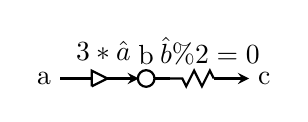
\begin{tikzpicture}[>=stealth]
  \draw (-.7,0) node [thin]{a};
    %  \draw [->,thick,dashed] (-.3,0) -- ++(.8,0);
    \begin{scope}[xshift=-14 pt]
    \draw [-, thick] (0,0) -- (0.4,0);
           \draw [-, thick] (0.4, -0.1) -- (0.4, 0.1) -- (0.6, 0) --(0.4, -0.1);
           \draw [->, thick](0.6,	0) -- (1,0);
           \draw (.55, .35) node [thin] {$3*\hat{a}$};
      \end{scope}
      \draw ++(.6,.3) node [thin]{b};
      \draw [thick] (.6,0) circle (3pt);
      \draw ++(.75,.25) node [thin]{};%c
      \draw ++(2.1,0) node [thin]{c};
      \draw [thick](0.7,0) -- (.9,0);
      \begin{scope}[xshift=23pt]
 \draw [-, thick] (-.1,0) -- (0.25,0) -- (0.3, -0.1) -- (0.4, 0.1) -- (0.5, -0.1) -- (0.6, 0.1) --(0.65, 0);
       \draw [->, thick](0.65,0) -- (1.1,0);
       \draw (.6, .35) node [thin] {$\hat{b}\%2=0$};
      \end{scope}
     % \def\rectanglepath{-- ++(0, .1) -- ++(.5,0) -- ++(0,-.2) -- ++(-.5, 0) -- ++(0,.1) --cycle}
     % \draw [thick] (.9,0) \rectanglepath;
      %\draw [->,thick] (1.4,0) --++(.25,0);
%
%      \draw [thick] (.6,0) circle (3pt);
%      \draw ++(.75,.15) node [thin]{e};
%      \draw ++(2,0) node [thin]{f};
%      \begin{scope}[yshift=-15 pt,xshift=-10 pt,rotate=25]
%     %  \draw (-.2,0) node [thin]{c};
%       \draw (1.2,.35) node [thin]{b};
%       \draw [-, thick] (0,0) -- (0.4,0);
%       \draw [-, thick] (0.4, -0.1) -- (0.4, 0.1) -- (0.6, 0) --(0.4, -0.1);
%       \draw [->, thick](0.6,	0) -- (1,0);
%       \draw (.55, .35) node [thin] {$3*\hat{c}$};
%       \end{scope}
%       \begin{scope}[yshift=15 pt,xshift=-10 pt,rotate=-25]
%       \draw (-.2,0) node [thin]{a};
%      % \draw (1.2,-.35) node [thin]{d};
%       \draw [-, thick] (0,0) -- (0.4,0);
%       \draw [-, thick] (0.4, -0.1) -- (0.4, 0.1) -- (0.6, 0) --(0.4, -0.1);
%       \draw [->, thick](0.6,0) -- (1,0);
%       \draw (.55, .35) node [thin] {$2*\hat{a}$};
%       \end{scope}
%       \begin{scope}[xshift=23 pt]
%       \draw [-, thick] (-.1,0) -- (0.25,0) -- (0.3, -0.1) -- (0.4, 0.1) -- (0.5, -0.1) -- (0.6, 0.1) --(0.65, 0);
%       \draw [->, thick](0.65,0) -- (1.1,0);
%       \draw (.6, .35) node [thin] {$\hat{e}\%2=0$};
%       \end{scope}
    \end{tikzpicture}
              \caption{A data-aware Reo connector}
                     \label{fig:examplereo1}   
   \end{figure}
   
  Since none of the Reo primitives in Figure \ref{fig:examplereo1} is context-dependent, we use the constraints corresponding to the primitives in this network as defined in Table \ref{tab:scfdfencodingsrcsp}.
  
   %\begin{table}[!t]
    \begin{equation}
       \label{eq:ex1line1}
       \psi_{Transformer}(a,b,3*\hat{a})=\tilde{a}\Leftrightarrow\tilde{b}\wedge\tilde{a}\Rightarrow(\hat{a}\in Number\wedge \hat{b}=3*\hat{a}))
       \end{equation} %\vspace{-.8cm}\\
         % \begin{equation}
          %\label{eq:ex1line2}
          %\psi_{Transformer}(c,d, 3*\hat{c}) = \tilde{c} \Leftrightarrow  \tilde{d} \wedge  (\tilde{c} \Rightarrow (\hat{a} \in Number \wedge \hat{d}=3*\hat{c})) 
          %\end{equation}  \vspace{-.8cm}\\
           %  \begin{equation}
            % \label{eq:ex1line3}
            % \parbox{10cm}{$\psi_{Merger}(b,d,e) = \tilde{e} \Leftrightarrow (\tilde{b} \vee  \tilde{d} ) \wedge \neg (\tilde{b} \wedge \tilde{d})  \wedge (\tilde{b} \Rightarrow (\hat{b}=\hat{e})) \wedge (\tilde{d} \Rightarrow (\hat{d}=\hat{e}))$}
           %  \end{equation}        \vspace{-.8cm}\\
         %  \begin{equation}
          %                 \label{eq:ex1line4}
           %                \parbox{10cm}{$\psi_{Filter} (e,f, \hat{e} \% 2=0) = \tilde{f} \Rightarrow (\tilde{e} \wedge \hat{e} \in Number \wedge (\hat{e} \% 2=0)) $}               
            %               \end{equation}
              \begin{equation}
                \label{eq:ex1line4}
                \psi_{Filter}(b,c,\hat{b}\%2=0)=\tilde{c}\Rightarrow(\tilde{b}\wedge\hat{b}\in Number\wedge(\hat{b}\%2=0))
                \end{equation} \\ %vspace{.8cm}\\
      % \end{table}       
       
   Equation \ref{eq:ex1line1} states that flow occurs on the source end of the \emph{transformer} channel iff it occurs on its sink end. In addition, flow can exist only if the data item that enters the source end of the channel is a number. In this case, the data item written on the sink end is three times the value of the source data item.  
   %     Equation \ref{eq:ex1line3} reflects the behavior of the \emph{merger}. It says that the sink end $e$ has flow iff  one and only one of its source ends $b$ or $d$ has flow. In this case, the data value passing through $e$ is the same as the data entering the source end with flow. 

   Equation \ref{eq:ex1line4} expresses that flow on the source end of the \emph{filter} channel leads to flow on its sink end, iff the data item belongs to the channel's accepting pattern (which is $\hat{b}\%2=0$). 
   
   In this case, the value of data items passing through the ends are equal. No flow through the sink end $c$ is either due to no flow on $b$ or that the incoming data item does not satisfy the accepting pattern. As mentioned, the conjunction of these constraints (subject to Axiom \ref{ax:mixednode}, which trivially holds in this case) encodes the behavior of the given Reo network.

\subsection{Solving RCSPs}
In this section, we show how to obtain the solutions of RCSPs. 
%A solution $\mathcal{S}$ for a constraint $C$ is a function $\mathcal{S} : \mathcal{V} \rightarrow 2^\mathcal{D} \cup \{\top, \bot\}$ such that for all distinct $v_i \in \mathcal{V}, 1 \leq i \leq n = |\mathcal{V}|$, we have $z_i \in \mathcal{S}(v_i)$ implies $C\left[v_1, v_2, \dots, v_n \setminus z_1, z_2, \dots, z_n \right]$ is true.
%\end{definition}
Since Reo Constraint Satisfaction Problems (RCSPs) have predicates with free variables of types Boolean ($\{\top, \bot\}$) and data ($\mathcal{D}$), a SAT-solver or a numeric constraint solver cannot solve them alone. Satisfiability Modulo Theories (SMT) \cite{smt} solvers find solutions for propositional satisfiability problems where propositions are either Boolean or constraints in a specific theory. 

However, SMT-solvers are not applicable in our case either, because unlike SAT-solvers they find only an instance of a solution as opposed to the complete set of answers. Another drawback of most SAT- and SMT-solvers is that they work only on quantifier-free formulae, while we use existential quantifies to implement the \emph{hiding} operator of constraint automata (see Section \ref{sec:hiding}).

To generate the CASM corresponding to a given Reo network, we need all solutions and thus resort to a hybrid approach that uses both SAT-solvers and Computer Algebra Systems (CASs), namely, REDUCE \cite{ReduceBook}, which is a system for general algebraic computations.

First, we form a pure Boolean constraint system by substituting data dependent constraints with new Boolean variables and find all solutions for the new constraints using a SAT-solver. Then, by substituting each such solution into the original constraints, we obtain a data dependent  constraint satisfaction problem that a CAS can solve symbolically. From these solutions, we extract a CASM corresponding to the Reo network encoded by the original set of constraints. Our approach avoids state explosion by treating data constraints symbolically. In the following, we elaborate on our approach.

In an RCSP $\langle \mathcal{P}, \mathcal{M}, M_0, \mathcal{V}, C \rangle$, let $\mathcal{V}_B$ and $\mathcal{V}_D$ be the sets of free Boolean and free data variables of $C$, respectively, where $\mathcal{V} = \mathcal{V}_B \cup \mathcal{V}_D$, and  let $A_D$ be the set of atomic predicates of $C$ containing data variables. The following is our procedure for solving $C$.
\begin{enumerate}
\item We obtain $C_B$ from $C$ by replacing every occurrence of $x \in A_D$ with a unique new Boolean variable $y \notin \mathcal{V}$. For example, for $C=(\tilde{c} \Rightarrow  \tilde{b}) \wedge (\tilde{c} \Rightarrow (\hat{b} \in Number \Rightarrow \hat{b} \% 2=0))$ in Figure \ref{fig:examplereo1}, we obtain $C_B$ as $(\tilde{c} \Rightarrow  \tilde{b}) \wedge (\tilde{c} \Rightarrow (y_1 \Rightarrow y_2))$  where $y_1$ and $y_2$ replace $\hat{b} \in Number$ and $\hat{b} \% 2=0$, respectively.
\item An off-the-shelf SAT-solver can find the set of solutions $S_B$ for $C_B$. We define the finite set of constraints $C\left[S_B\right]=\{C\left[v_1, v_2, \dots, v_n \setminus z_1, z_2, \dots z_n\right]~|~ $ for all distinct $v_i \in \mathcal{V}_B, 1 \leq i \leq n = |\mathcal{V}_B|, z_i \in S \left( v_i \right), S \in S_B \}$. 
\item Every $C_D \in C\left[S_B\right]$ is a numerical constraint satisfaction problem, which we (symbolically) solve using a Computer Algebra System. Every solution to each $C_D$ along with the SAT solution $S \in \mathcal{S}_B$ that produced $C_D \in C\left[S_B\right]$ in the previous step, constitute a solution to the RCSP. 
\end{enumerate}

Using the presented technique, we obtain the solutions for the RCSP corresponding to Examples \ref{ex:noncontextsen} as follows: 

\begin{enumerate}
\label{eq:solutionex1}
%size	
%\item $\langle\{\tilde{a}=\bot, \tilde{b}=\bot, \tilde{c}=\bot, \tilde{d}=\bot, \tilde{e}=\bot, \tilde{f}=\bot, \mathring{m}=\bot, \mathring{m}'=\bot\}, \top\rangle$,
%\item $\langle\{\tilde{a}=\top, \tilde{b}=\top, \tilde{c}=\bot, \tilde{d}=\bot, \tilde{e}=\top, \tilde{f}=\bot, \mathring{m}=\bot, \mathring{m}'=\top\}, \hat{a}=\hat{b} \wedge \hat{b}=\hat{e} \wedge \hat{m}'=\hat{e}\rangle$,
%\item $\langle\{\tilde{a}=\bot, \tilde{b}=\bot, \tilde{c}=\top, \tilde{d}=\top, \tilde{e}=\top, \tilde{f}=\bot, \mathring{m}=\bot, \mathring{m}'=\top\}, \hat{c}=\hat{d} \wedge \hat{d}=\hat{e} \wedge \hat{m}'=\hat{e}\rangle$,
%\item $\langle\{\tilde{a}=\bot, \tilde{b}=\bot, \tilde{c}=\bot, \tilde{d}=\bot, \tilde{e}=\bot, \tilde{f}=\bot, \mathring{m}=\top, \mathring{m}'=\top\}, \hat{m}=\hat{m}'\rangle$,
%\item $\langle\{\tilde{a}=\bot, \tilde{b}=\bot, \tilde{c}=\bot, \tilde{d}=\bot, \tilde{e}=\bot, \tilde{f}=\top, \mathring{m}=\top, \mathring{m}'=\bot\}, \hat{m}=\hat{f}\rangle$.
\item $\langle\{\tilde{a}=\bot, \tilde{b}=\bot, \tilde{c}=\bot\}, \top\rangle$,
\item $\langle\{\tilde{a}=\top, \tilde{b}=\bot, \tilde{c}=\bot\}, \hat{a} \not \in Number\rangle$,
\item $\langle\{\tilde{a}=\top, \tilde{b}=\top, \tilde{c}=\bot\}, \hat{a} \in Number \wedge \hat{b}=3*\hat{a}\ \wedge \ \hat{b} \%2\neq 0\rangle$,
\item $\langle\{\tilde{a}=\top, \tilde{b}=\top, \tilde{c}=\top\},\hat{a} \in Number \wedge \ \hat{b}=3*\hat{a}\ \wedge \ \hat{b}\%2=0\ \wedge \ \hat{b}=\hat{c}\rangle$.
\end{enumerate} %\vspace*{-.4cm}

\begin{figure}[!h]
   \centering
      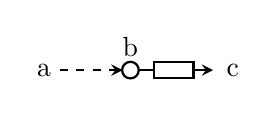
\begin{tikzpicture}[>=stealth]
      \draw (-.5,0) node [thin]{a};
      \draw [->,thick,dashed] (-.3,0) -- ++(.8,0);
      \draw ++(.6,.3) node [thin]{b};
      \draw [thick] (.6,0) circle (3pt);
      \draw ++(.75,.25) node [thin]{};%c
      \draw ++(1.9,0) node [thin]{c};
      \draw [thick](0.7,0) -- (.9,0);
      \def\rectanglepath{-- ++(0, .1) -- ++(.5,0) -- ++(0,-.2) -- ++(-.5, 0) -- ++(0,.1) --cycle}
      \draw [thick] (.9,0) \rectanglepath;
      \draw [->,thick] (1.4,0) --++(.25,0);
    \end{tikzpicture}
    \caption{A context-dependent Reo connector}
    \label{fig:lossyfifocam}
   \end{figure}  

\begin{BehExample}
\label{ex:contextsenniaz}
Figure \ref{fig:lossyfifocam} depicts a Reo network that consists of a \emph{lossySync} channel and a \emph{FIFO$_1$} channel connecting on the node $b$.    
\end{BehExample}

Since the Reo network in Figure \ref{fig:examplereo1} contains a \emph{lossySync} that is a context dependent channel, we use the context-aware RCSP encoding from Table \ref{tab:contextencoding}: %as follows:

%\begin{table}[!ht]
\begin{equation}
\label{eq:ex1line5}
%\parbox{10cm}{$
\psi_{LossySync}(a, b) = \tilde{b} \Rightarrow (\tilde{a} \wedge (\hat{a}=\hat{b})) \wedge \neg {a^c}^\triangleright \wedge \neg \tilde{a} \Rightarrow {b^k}^\triangleright. 
%$}
\end{equation} \\
\begin{equation}
\label{eq:ex1line7}
\parbox{.99\columnwidth}{$\psi_{FIFO_{1}}(b, c, m)  = \tilde{b} \Rightarrow (\neg \mathring{m} \wedge \mathring{m}' \wedge (\hat{m}'=\hat{b})) \wedge \tilde{c} \Rightarrow (\mathring{m} \wedge \neg \mathring{m}' \wedge (\hat{m}=\hat{c})) \wedge (\neg \tilde{b} \wedge \neg \tilde{c}) \Rightarrow ((\mathring{m} \Leftrightarrow \mathring{m}') \wedge \mathring{m} \Rightarrow (\hat{m}=\hat{m}')) %reasin
\wedge \neg \mathring{m} \Rightarrow {c^c}^\triangleright \wedge  \mathring{m} \Rightarrow {b^k}^\triangleright.
 $}
\end{equation}
%\end{table}


Equation \ref{eq:ex1line5} states that flow on the sink end of the \emph{lossySync} is due to flow on its source end. If there is flow on the sink end of the \emph{lossySync}, the data items exchanged at the source and the sink ends are the same. However, it is possible that the source end has  flow, but the sink end does not. In this case, the reason for no flow comes from the environment with which the sink end communicates. The third possible behavior of the channel is that there is no flow on the source end due to the environment, in which case the channel provides a reason for no flow on its sink end.
%Equation \ref{eq:ex1line6} states that there is flow on the source end of the \emph{replicator} iff there is flow on its sink end. In this case, the data item exchanged on the ends are the same. However, in the case of no flow, the reason for no flow originates from the environment.
%%%TODOwhat about colros

Equation \ref{eq:ex1line7} expresses the behavior of  the \emph{FIFO}$_1$ channel as follows: The flow on the source end of the channel states that the value of the variable representing the state memory (of the current state) is undefined. The flow on the source end defines the state memory variable for the next state to contain the value of the incoming data item. On the other hand, flow on the sink end means that the value of the state memory variable is defined. The data item leaving the sink end is equivalent to the buffer's data item. In addition, the value of the state memory variable becomes undefined in the next state. If there is no flow on the ends, the variables related to the states stay the same. Being empty, the \emph{FIFO}$_1$ channel provides a reason for no flow on its sink end, while being full does so on the source end of the channel.

The solutions for the RCSP \ref{eq:ex1line7}, (where for brevity, we omit the values of the variables representing the context, such as ${b^c}^\triangleright$) are as follows:

\begin{enumerate}
\label{eq:solutionex2}
\item $\langle\{\tilde{a}=\bot, \tilde{b}=\bot, \tilde{c}=\bot, \mathring{m}=\bot, \mathring{m}'=\bot\}, \top\rangle$,
\item $\langle\{\tilde{a}=\top, \tilde{b}=\top, \tilde{c}=\bot, \mathring{m}=\bot, \mathring{m}'=\top\},  \hat{a}=\hat{b} \wedge \hat{m}'=\hat{b}\rangle$,
\item $\langle\{\tilde{a}=\top, \tilde{b}=\bot, \tilde{c}=\bot, \mathring{m}=\top, \mathring{m}'=\top\}, \hat{m}=\hat{m}'\rangle$,
\item $\langle\{\tilde{a}=\bot, \tilde{b}=\bot, \tilde{c}=\bot, \mathring{m}=\top, \mathring{m}'=\top\}, \hat{m}=\hat{m}'\rangle$,
\item $\langle\{\tilde{a}=\top, \tilde{b}=\bot, \tilde{c}=\bot, \mathring{m}=\top, \mathring{m}'=\bot\},  \hat{m}=\hat{c}\rangle$,
\item $\langle\{\tilde{a}=\bot, \tilde{b}=\bot, \tilde{c}=\top, \mathring{m}=\top, \mathring{m}'=\bot\}, \hat{m}=\hat{c}\rangle$.
\end{enumerate}

\subsection{Constructing CASM}
In order to construct the CASM from the set of solutions $S$ for an RCSP $\langle \mathcal{P}, \mathcal{M}, M_0,  \mathcal{V}, C \rangle$, we first define

\begin{itemize} 
  \item $\N = \{n~|~ n^c \in \mathcal{P} \vee n^k \in \mathcal{P} \}$
\end{itemize} 

and then map each solution $\langle s, s_d \rangle \in S$ into a transition $\longtransition{q}{N, g}{p}$ as follows: %explained in the procedure $genTrnas$. 
%\noindent
%\emph{The $genTrnas$ procedure:}
\begin{itemize}
%\item The start and the target states of the transition $t$, $q$ and $p$, respectively are identified by their sets of state memory variables as $ \mathring{m} in q $ iff $ s(\mathring{m})=\top $ and $ \mathring{m}' in p $ iff $ s(\mathring{m})=\top$.
\item $q = \langle\{m ~|~ m \in \mathcal{M}, s\left(\mathring{m}\right) = \top \}\rangle$,
\item $p = \langle\{m ~|~ m \in \mathcal{M}, s\left(\mathring{m}'\right) = \top \}\rangle$,
%\item $\mathcal{N} = \{n ~|~ n^c \in \mathcal{P} \vee n^k \in \mathcal{P} \}$,
\item $N =  \{ n ~|~ n \in \mathcal{N}, s\left(\tilde{n}\right) = \top \}$,%\{ n ~|~ n_c \in \mathcal{P} \vee n_k \in \mathcal{P}, s\left(\tilde{n}\right) = \top \}$,
\item The data constraint $g$ is (a syntactic variant of) $s_d$. 
\end{itemize} 

We obtain the CASM $A=\left( Q, \mathcal{N}, \rightarrow, q_0, \mathcal{M} \right)$ from the set $\longrightarrow$ of all transitions generated above, where: %$T$ that the $genTrans$ produces, such that:
 \begin{itemize}
\item $Q = \{q ~|~ \longtransition{q}{N, g}{p} \vee \longtransition{p}{N, g}{q} \}$, 
\item $q_0 = \langle\{m~|~ m \in M_0, s(\mathring{m}) = \top \}\rangle$, 
%is the state with the state memory variables like $m$ that $s_{b0}(\mathring{m})=\top$ and $s_{b0}$ is the first calculated solution for $C_B$,
%\item $\rightarrow$ is the set of all transitions, $T$,
\item $\mathcal{M}$ is the same $\mathcal{M}$ as in the RCSP.
 \end{itemize}

Applying the above procedure to the solutions of RCSPs constraints generates their corresponding CASMs. For instance, the first solution for the constraints in Example \ref{ex:noncontextsen} generates the transition $\longtransition{q}{\emptyset, true}{q}$, where $q$ is the only state of the CASM, which has no state memory variable. This is so because the set of variables of the form $\mathring{m}$ is empty. Also, the transition has no synchronizing port, because the value of every one of the variables $\tilde{a}, \tilde{b}$ and $\tilde{c}$ is $\bot$. Figures \ref{fig:goodcaex1} and \ref{fig:goodcaex2} show the CASMs derived from the RCSPs in Examples \ref{fig:examplereo1} and \ref{fig:lossyfifocam}.

% \vspace*{-.5cm}
%\noindent
\begin{figure}[t]
        \subfloat{%[????CASM of Example \ref{ex:noncontextsen}????]{
                \centering
                %\scalebox{0.7}{
                \begin{tabular}{c}
		    %  
		      \tikz{
				  \node[state,minimum size=5mm] (q) {};%, initial
			      \path[transition] (q) edge [loop above,looseness=25] node [text width=1cm,align=center,above]  {$\emptyset,\textit{true}$} (q); 
			      \path[transition] (q) edge [loop left,looseness=25] node [left,text width=2.1cm,align=right] {$\{a, b, c\},$\\ $\hat{a} \in Number \wedge$ \\$\hat{b}=3*\hat{a}\ \wedge$\\ $\hat{b}=\hat{c}\ \wedge$ \\ $\hat{b}\%2=0$}  (q); 
			      \path[transition] (q) edge [loop right,looseness=25] node [right,text width=2.1cm,align=left] {$\{a,b\},$\\$\hat{a} \in Number \wedge$ \\ $\hat{b}=3*\hat{a}\ \wedge$\\ $\hat{b} \%2\neq 2$}  (q);
			      \path[transition] (q) edge [loop below,looseness=25,text width=2.5cm,align=center] node [below]  {$\{a\},\hat{a} \not \in Number$} (q); 
			   %   \path[transition] (q) edge  node [above] {$\{f\}, \hat{m}=\hat{f}$}  (q);                           
		      }                  		    
                \end{tabular}
	%	}
	 %       \caption{}%CASM of Example \ref{ex:noncontextsen}}
		\label{fig:goodcaex1}
        }
        \\ 
	\subfloat{%[h]{0.95\textwidth}
                \centering
                %\scalebox{0.7}{
                \begin{tabular}{c}
		    %  
		      \tikz{
			    \node[state] (q) {m};
			    \node[state, left of=q, node distance=3cm, initial] (p) {};
			    \path[transition] (q) edge [loop right] node[above] {$\ \ \ \ \ \ \emptyset, \textit{true}${}} (q); 
			    \path[transition] (q) edge [bend left=50] node[below]  {$\ \ \ \ \ \ \ \ \ \ \ \{a,b,c\}, \hat{a}=\hat{b} \wedge \hat{b}=\hat{c} \wedge \hat{m}'=\hat{c}$}  (p);  
			    \path[transition] (p) edge [loop above] node[left]  {$\{a\},\textit{true}${}} (p); 
			    \path[transition] (p) edge [loop below] node[left]  {$\emptyset,\textit{true}$}  (p);     
			    \path[transition] (p) edge  node[above]  {$\{a,d\}, \hat{m}=\hat{d}$}  (q);                  
			    \path[transition] (p) edge [bend left=50] node[above]  {$\{d\}, \hat{m}=\hat{d}$}  (q);
                  }  	
		  \end{tabular}
		%}
	     %   \caption{}%CASM of Example \ref{ex:contextsen}}
		\label{fig:goodcaex2}
        }	
   \caption{CASMs generated for Figures \ref{fig:examplereo1} and \ref{fig:lossyfifocam}}
   \label{lblmail}
\end{figure}

Our approach deals with data in a symbolic fashion, where we partition the global set of data values to equivalence classes toward which a Reo network behaves differently. This is in contrast with the traditional way of dealing with data in the formal semantics of Reo (and other models), where they consider a different state for each possible value that can be stored in buffers and a distinct transition for each data value passing through the ports. 

Our symbolic approach allows working with an infinite data domain. In addition, rather than implementing the highly time- and memory-demanding custom-made algorithms to generate Reo formal semantics, we use the efficient SAT-solvers and computer algebra systems to solve constraints whose solutions are equivalent to these models. 

An experimental study done on the efficiency of using SAT-solvers to generate Reo formal semantics \cite{JoseThesis} compares two prototypes based on constraint satisfaction techniques and connector coloring semantics, without taking data constraints in consideration. The results illustrate that the approach based on constraint solving scales better and is more efficient. In chapter \ref{ch:prio} we present an evaluation through a case study, which affirms this conclusion.


\begin{figure}[t]
 \centering
 %\begin{tabular*}{\linewidth}{ c   c } %@{\extracolsep{\fill}} 
%CC %\hline
         %\begin{sub figure}{0.9\columnwidth}{
   %      \raisebox{3.6cm}[5cm]{
         %\vspace{1cm}
             \begin{tikzpicture}[->,>=stealth',shorten >=1pt,auto,node distance=1.5cm,semithick]
               \node[state] (s1) [initial] at (0,0) {};
               \node[state] (s2) [right of=s1] {m};
               \path (s1) edge [loop below] node [left] {$\{A\}, true\ \ $} (s1);
               \path (s1) edge [bend left] node [above,text width=30mm]{$\ \ \ \ \ \ \ \ \ \ \{A,B\},\ \ $\\$d_A=d_B \wedge d_A=m'$\\$\ $} (s2)
                     (s2) edge [bend left] node [below,swap,text width=12mm] {$\ $\\$\ \ \ \{C\},\ \ $\\$d_C=m$} (s1)
                     (s2) edge [loop below] node [right] {$\ \ \ \{A\}, true\ \ $} (s2);
             \end{tikzpicture}
			\caption{CASM for Figure \ref{fig:lossyfifocam}}
			\label{fig:cccasma}
        \end{figure}    

        
        \begin{figure}[t]
              \begin{tikzpicture}[->,>=stealth',shorten >=1pt,auto,node distance=1.5cm,semithick]
                 \tikzstyle{every path}=[thick]
                  \begin{scope} [start chain=1, node distance=-0.15mm] %, going right    
                 \node (first) at (1,0) {
                    $\begin{matrix}  
                     & A_c &B_k &B_c&C_k \\ 
                    \Romanbar{1} &\triangleright&\triangleright&\triangleleft&\triangleright \\
                    \Romanbar{2} &\triangleright&\triangleleft&\triangleleft&\triangleright \\
                    \Romanbar{3} &-&-&-&\triangleright \\
                                 &              & L_0        &             &  \\
                    \end{matrix}$};
                    \node (second) at (7,0) {
                     $ \begin{matrix} 
                         &A_c &B_k &B_c&C_k \\
                        1 &\triangleright&\triangleright&\triangleleft&\triangleleft \\
                    	2 &\triangleright&\triangleleft&\triangleleft&\triangleleft \\
                    	3 &\triangleright&\triangleright&\triangleleft&- \\
                    	4 &\triangleright&\triangleright&\triangleleft&- \\
                    	  &              & L_1        &             &  \\
                        \end{matrix} $	 
                    };
                    \draw[->](second.north west) to [bend right=25] node [auto,swap] {$3$} (first.north east);
                    \draw[->](second.south west) to [bend left=25] node [auto] {$4$} (first.south east);
                    \draw[->](first) to node [auto] {$\Romanbar{3}$} (second); 
					\draw[->](first.north)  .. controls (-1,2) and (3,2) .. node [auto] {$\Romanbar{1}$} (first.north);
					\draw[->](first.west)   .. controls (-2,-2) and (-2,2) .. node [auto] {$\Romanbar{2}$} (first.west);
					\draw[->](second.east)  .. controls (9.5,2) and (9.5,-2) .. node [auto] {$2$} (second.east);
					\draw[->](second.north) .. controls (9,2) and (5,2) .. node [auto,swap] {$1$} (second.north);
                   \end{scope}        
               \end{tikzpicture}       
          \caption{CC for Figure \ref{fig:lossyfifocam}}
          \label{fig:ccandcasm}
         \end{figure}

\section{Hiding}
\label{sec:hiding}
We use \emph{hiding} to abstract from internal transitions. This is a mechanism to support hierarchy and is used to create components. 

The author in \cite{JoseThesis} proposes applying the existential quantifier to the constraints encoding of the behavior of a network to abstract from internal ports and their corresponding data variables. Similarly, we use existential quantifiers such as $\exists \tilde{e}, \hat{e}, {e}^\triangleright:C$, where $C$ is the RCSP of a Reo network and $e$ is an internal node to hide.

Although several algorithms exist for the problem of quantifier elimination in Boolean algebra and first order logic \cite{quantifiedbool} \cite{ayari2002qubos} \cite{reduce}, we are not aware of any working tool that does quantifier elimination on Boolean algebraic formulae. Therefore, our tool implements the \emph{hiding} operator as defined for CASM.

Hiding the internal nodes on some transitions can make the set of their synchronized nodes empty. Here, we refer to such a transition as an \emph{empty} transition, if the free variables of its guard are merely state memory variables. Under some circumstances, we can merge the source and the target states of empty transitions. Let $q$ and $p$ be two states in a CASM such that $\longtransition{q}{\emptyset, g}{p}$. The following are the conditions under which the state $p$ can merge into the sate $q$:
\begin{enumerate}
 \item The states $q$ and $p$ have the same number of state memory variables.
 \item The guard $g$ consists of the conjunction of the predicates of the form of $x = y'$, for $x, y \in \mathcal{M}$. This way, $g$ defines a correspondence relation between the state memory variables of the state $q$ and those of the state $p$. %Here, we define $g[n] = m$, if $g$ contains $m = n'$. 
 \item For each transition $\longtransition{q}{N, g'}{r}$ where $r \notin \{p,q\}$, there is a transition $\longtransition{p}{N, g''}{r}$ such that $g' \Leftrightarrow g''_g$, where $g''_g$ is obtained from $g$ by replacing all occurrences of the next state memory variable $y'$ with the next state memory variable $x'$, if $g$ contains $x=y'$ for state memory variables $x, y \in \mathcal{M}$.
 \item For each transition $\longtransition{r}{N, g'}{p}$ where $r \notin \{p,q\}$, there is a transition $\longtransition{r}{N, g''}{q}$ such that $g'' \Leftrightarrow g'_g$, where $g'_g$ is derived from $g$ by substituting all occurrences of the state memory variable $x$ in $g$ with the state memory variable $x$, if $g$ contains $x=y'$ for state memory variables $x, y \in \mathcal{M}$.
\end{enumerate}

Provided that the above conditions hold, the state $p$ merges into the state $q$ as follows:
\begin{enumerate}
 \item We eliminate the transition $\longtransition{q}{\emptyset, g}{p}$. 
 \item We remove the state $p$ after substituting $y$, $y'$, and $p$ with $x$, $x'$, and $q$ in all transitions. Observe that such substitutions convert the non-eliminated transitions between the states $q$ and $p$ into loops over the state $q$.
 \end{enumerate}
\begin{BehExample}
\label{ex:bisimfifos}
Figure \ref{fig:example2fifos} shows a \emph{FIFO$_2$} derived from composing two \emph{FIFO$_1$}s. The CASM corresponding to the \emph{FIFO$_2$} is in Figure \ref{fig:extrastatefifos}. Figure \ref{fig:extrastatefifoshide} depicts the CASM resulting from hiding the mixed node $b$. Figure \ref{fig:extrastatefifoshidemerged} presents the result of eliminating the empty transitions.

\begin{figure}[t]
  \centering
  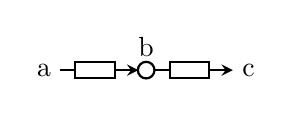
\begin{tikzpicture}[>=stealth]
  \def\rectanglepath{-- ++(0, .1) -- ++(.5,0) -- ++(0,-.2) -- ++(-.5, 0) -- ++(0,.1) --cycle}
        \draw (-.7,0) node [thin]{a};
	\draw [thick](-.5,0) -- ++(.2,0);     
	\draw [thick] (-.3,0) \rectanglepath;
	\draw [->,thick] (.2,0) --++(.3,0);
	\draw ++(.6,.3) node [thin]{b};
	\draw [thick] (.6,0) circle (3pt);
	\draw ++(.75,.25) node [thin] {};
	\draw ++(1.9,0) node [thin]{c};
	\draw [thick](0.7,0) -- (.9,0);     
	\draw [thick] (.9,0) \rectanglepath;
	\draw [->,thick] (1.4,0) --++(.3,0);
  \end{tikzpicture}
  \caption{Two FIFO$_1$s forming FIFO$_2$}
  \label{fig:example2fifos}
\end{figure}
\end{BehExample}

\begin{figure}[H]
                \centering
    \subfloat[CASM of Figure \ref{fig:example2fifos}]{    %\begin{sub figure}[b]{\columnwidth}
                \centering
                \begin{tabular}{c}
		     %\vspace{1cm} 
		     \tikz{
			  \node[state, initial] (q) {\parbox[top][][c]{.5cm}{}};
			  \node[state, right of=q, node distance=5cm] (p) {\parbox{.5cm}{ $\ m$}};
			  \node[state, below of=q, node distance=3.5cm] (r) {\parbox{.5cm}{ $\ \ n$}};
			  \node[state, right of=r, node distance=5cm] (s) {\parbox{.9cm}{ $\ m,  n$}};
			  %transitions
			  \path[transition] (q) edge [loop above] node [left] {$\emptyset, true\ $} (q); 
			  \path[transition] (p) edge [loop right] node [above] {$\ \emptyset, true$} (p); 
			  \path[transition] (r) edge [loop left] node [below] {$\emptyset, true\ $} (r); 
			  \path[transition] (s) edge [loop right] node [above] {$\ \emptyset, true$} (s); 
			  \path[transition] (q) edge [] node [above,text width=2cm,align=center] {$\{a\},\ m'=\hat{a}$} (p);     
			  \path[transition] (p) edge [bend left] node [] {\parbox{3.75cm}{ $\{b\},\ \hat{b}=m \wedge \ n'=\hat{b}$}}  (r);   
			  \path[transition] (r) edge [] node [below,text width=3.5cm,align=center]{$\{a\},\ m'=\hat{a} \wedge \ n'=n$}  (s);
			  \path[transition] (s) edge [] node [right] {\parbox{2cm}{$\{c\},\ m'=m \\ \wedge \ \hat{c}=n$}}  (p);
			  \path[transition] (r) edge [] node [left] {$\{c\},\ \hat{c}=n$}  (q);
			  \path[transition] (r) edge [bend left] node [] {\parbox{3.5cm}{ $\{a,c\},\ m'=\hat{a} \ \wedge \hat{c}=n $}}  (p);   
		      }\\                  
		\end{tabular}
            %    \caption{CASM of Figure \ref{fig:example2fifos}}
		\label{fig:extrastatefifos}
    }%    \end{sub figure}%
      %  \ %add desired spacing between images, e. g. ~, \quad, \qquad etc. 
          %(or a blank line to force the sub figure onto a new line)
          
          \centering
      \subfloat[Hiding internal ports]{ % in Figure??????~\label{fig:extrastatefifos} \begin{sub figure}[b]{\columnwidth}
                \centering
		\begin{tabular}{c}
		  \tikz{
			\node[state, initial] (q) {\parbox[top][][c]{.5cm}{}};
			\node[state, right of=q, node distance=5cm] (p) {\parbox[top][][c]{.5cm}{ $\ m$}};
			\node[state, below of=q, node distance=3.5cm] (r) {\parbox[top][][c]{.5cm}{ $\ \ n$}};
			\node[state, right of=r, node distance=5cm] (s) {\parbox[top][][c]{1cm}{ $\ m, n$}};
			%transitions
			\path[transition] (q) edge [loop above] node [left] {$\emptyset, true\ $} (q); 
			\path[transition] (p) edge [loop right] node [above] {$\ \ \ \ \ \emptyset, true$} (p); 
			\path[transition] (r) edge [loop left] node [above] {$\emptyset, true\ \ \ \ \ $} (r); 
			\path[transition] (s) edge [loop right] node [above] {$\ \ \emptyset, true$} (s);
			\path[transition] (q) edge [] node [above,text width=2cm,align=center] { $\{a\},$\ $m'=\hat{a}$} (p);     
			\path[transition] (p) edge [bend left] node [] {\parbox{1.5cm}{ $\emptyset,\ n'=m$}}  (r);   
			\path[transition] (r) edge [] node [below,text width=5cm,align=center] {$\{a\},$\ $m'=\hat{a} \wedge$\    $n'=n$}  (s);
			\path[transition] (s) edge [] node [right] {\parbox{2cm}{ $\{c\},\ m'=m \\ \wedge \ \hat{c}=n$}}  (p);
			\path[transition] (r) edge [] node [left] {$\{c\},\ \hat{c}=n$}  (q);              	
			\path[transition] (r) edge [bend left] node [] {$\{a,c\},\ m'=\hat{a}\ \wedge\ \hat{c}=n$}  (p);   
		  }                 
		\end{tabular}
            %    \caption{Hiding internal ports}% in Figure~\label{fig:extrastatefifos}}
                \label{fig:extrastatefifoshide}
        }%\end{sub figure}
        %\ %add desired spacing between images, e. g. ~, \quad, \qquad etc. 
          %(or a blank line to force the sub figure onto a new line)
          
          \centering
        \subfloat[Merging the states]{%[b]{0.99\columnwidth}
                %\centering
               \hspace*{-2cm} \begin{tabular}{c}
		      \tikz{
			      \node[state, initial] (q) {\parbox[top][][c]{.5cm}{}};
			      \node[state, right of=q, node distance=2.75cm] (p) {\parbox[top][][c]{.5cm}{ $\ m$}};
			      \node[state, right of=p, node distance=2.75cm] (s) {\parbox[top][][c]{.5cm}{ $\ m,\\ \ \ n$}};
			      \path[transition] (q) edge [loop above,looseness=25] node [above,text width=1cm,align=center] {$\emptyset,\ true\ $} (q); 
			      \path[transition] (p) edge [loop below,looseness=20] node [below,text width=2cm,align=center] {$\emptyset,\ true\ $} (p); 
			      \path[transition] (s) edge [loop above,looseness=15] node [above,text width=1cm,align=center] {$\emptyset,\ true\ $} (s); 
			      \path[transition] (q) edge [bend left] node [above] {\parbox{1.15cm}{ $\ \{a\}, \\ m'=\hat{a}$}} (p);     
			      \path[transition] (p) edge [bend left] node [above] {\parbox{1.5cm}{ $\ \ \ \{a\}, \\ m'=\hat{a} \wedge \\ \ \ n'=m$}}  (s);
			      \path[transition] (s) edge [bend left] node [below,text width=4.2cm,align=right] { $\ \ \ \ \ \ \ \ \{c\},$  $m'=m \wedge$ $\hat{c}=n$}  (p);
			      \path[transition] (p) edge [bend left] node [below] {\parbox{1.15cm}{$\ \{c\}, \\ \hat{c}=m$}}  (q);
			      \path[transition] (p) edge [loop above,looseness=25] node [above] {\parbox{2.5cm}{ $\{a,c\}, m'=\hat{a} \wedge \\ \hat{c}=m$}}  (p);
		      } 
	      \end{tabular}
            %  \caption{Merging the states}% in Figure \ref{fig:extrastatefifoshide}}
              \label{fig:extrastatefifoshidemerged}
       }%\end{sub figure}
     %  {\caption{Hiding the empty transition and merging its source and target states for the CASM of FIFO$_2$ in Figure \ref{fig:example2fifos}}}
    \caption[Hiding the empty transition]{Hiding the empty transition and merging its source and target states for the CASM of FIFO$_2$ in Figure \ref{fig:example2fifos}}
        \label{fig:animals}
\end{figure}

\section{Correctness and compositionality}
\label{sec:proofs}
CASM and CC model the presence and the absence of data flow on a Reo network at different levels of granularity. For instance, Figure \ref{fig:canodes} and Figure \ref{fig:ccports1} are the CASM and CC semantics for the Reo network in Figure \ref{fig:reonodes}. As the figures show, the node $b$ in CASM is mapped to three primitive ends in CC, which do not necessarily have the same coloring. 

In this section, we formally investigate the relation between the solutions of the RCSP for a given Reo network and its CC and CASM semantics. However, we first need to present some definitions. 



   \begin{figure}[t]
   \centering
      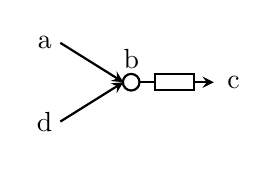
\begin{tikzpicture}[>=stealth]
      \draw (-.5,-.5) node [thin]{d};
      \draw [->,thick] (-.3,.5) -- ++(.8,-.5);
      \draw (-.5,.5) node [thin]{a};
      \draw [->,thick] (-.3,-.5) -- ++(.8,.5);
      \draw ++(.6,.3) node [thin]{b};
      \draw [thick] (.6,0) circle (3pt);
      \draw ++(.75,.25) node [thin]{};%c
      \draw ++(1.9,0) node [thin]{c};
      \draw [thick](0.7,0) -- (.9,0);
      \def\rectanglepath{-- ++(0, .1) -- ++(.5,0) -- ++(0,-.2) -- ++(-.5, 0) -- ++(0,.1) --cycle}
      \draw [thick] (.9,0) \rectanglepath;
      \draw [->,thick] (1.4,0) --++(.25,0);
    \end{tikzpicture}
    \caption{A sample Reo network}
    \label{fig:reonodes}
   \end{figure}      


    \begin{figure}[t]
    \centering
           \begin{tikzpicture}[->,>=stealth',shorten >=1pt,auto,node distance=5cm,semithick]
               \node[state, initial] (s1) at (0,0) {};
               \node[state] (s2) [right of=s1] {m};
               \path (s1) edge [bend left=70] node [above, text width=35mm]  {$\{a,b\},\ \hat{a}=\hat{b} \wedge \hat{m}'=\hat{b}$} (s2);
               \path (s1) edge [bend right] node [below,text width=30mm]  {$\ \{b,d\},\ \hat{b}=\hat{d} \wedge \hat{m}'=\hat{d}$} (s2)
                     (s2) edge [] node [above,swap,text width=18mm]  {$\{c\}, \hat{c}=\hat{m}$}   (s1);
             \end{tikzpicture}
     \caption{CASM corresponding to Figure \ref{fig:reonodes}}
     \label{fig:canodes}
    \end{figure}
 
 
    \begin{figure}[t]
    \centering
       \begin{tikzpicture}[>=stealth,decoration={triangles,amplitude=.4mm,segment length=2mm,post length=1mm,pre length=1mm}]]
      %\def\trianglepath{-- ++(0, .1) -- ++(.1,-.1) -- ++(-.1,-.1) --cycle}
      %\def\bktrianglepath{-- ++(0, .1) -- ++(-.1,-.1) -- ++(.1,-.1) --cycle}
       \draw (-.5,-.5) node [thin]{d};
       \draw [->,thick] (-.3,.5) -- ++(.8,-.5);
       \draw [->,color=gray,decorate,thick] (.5,0) -- ++(-.8,.5);
       \draw (-.5,.5) node [thin]{a};
       \draw [->,thick] (-.3,-.5) -- ++(.8,.5);
       \draw [-,very thick,color=gray] (-.3,-.5) -- ++(.8,.5);
       \draw ++(.6,.3) node [thin]{b};
       \draw [thick] (.6,0) circle (3pt);
       \draw ++(.8,.25) node [thin]{};%c
       \draw ++(2.1,0) node [thin]{c};
       \draw [thick](0.7,0) -- (.9,0);h
       \draw [-,very thick,color=gray] (.7,0) -- ++(.2,0);
       \def\rectanglepath{-- ++(0, .1) -- ++(.5,0) -- ++(0,-.2) -- ++(-.5, 0) -- ++(0,.1) --cycle}
       \draw [thick] (.9,0) \rectanglepath;
       \draw [->,thick] (1.4,0) --++(.5,0);
       \draw [->,color=gray,decorate,thick] (1.4,0) -- ++(.5,0);
     \end{tikzpicture}
     \caption{A coloring annotated state of the CC corresponding to Figure \ref{fig:reonodes}}
     \label{fig:ccports1}
    \end{figure}      

For a given network $R$ with $A=\left(Q, \mathcal{N}, \rightarrow, q_0, \mathcal{M}\right)$, its CASM and $C=\langle \mathcal{P}, \mathcal{L}, L_0, \eta \rangle$, its CC, we define the function $\mathit{O}_R: \mathcal{P} \rightarrow \mathcal{N}$ as it maps each CC port to its corresponding node in CASM. 
%TODO[example]

\begin{definition}[Correlation $\sim$]
\label{def:correl}
Let $A=\left(Q, \mathcal{N}, \rightarrow, q_0, \mathcal{M}\right)$ be a CASM and $C=\langle \mathcal{P}, \mathcal{L}, L_0, \eta \rangle$ be a CC. We define the relation $\sim : Q \times \mathcal{L}$, as follows:
\begin{itemize}
\item $q_0 \sim L_0$, if $\mathcal{N}=\bigcup_{p \in \mathcal{P}} \mathit{O}_R(p)$.
\item For each $p \in Q$ and $L' \in \mathcal{L}$, $p \sim L'$ if the following conditions hold: 
\begin{enumerate}
\item There exists $q \in Q$ and $L \in \mathcal{L}$ such that $\longtransition{q}{N,g}{p}$ and $L'=\eta(L, l)$, where $l \subset L$,
\item For all $n \in N, n = \mathit{O}_R(p) \Leftrightarrow l(e)=-$,
\item $q \sim \mathcal{L}$. 
\end{enumerate}
\end{itemize}

\noindent
If a relation $\sim$ exists between $Q$ and $\mathcal{L}$, then we say that $A$ correlates to $C$, written as $A \sim C$.
\end{definition}

It is easy to see that if $A$ and $C$ belong to the same Reo network, then $q_0 \sim L_0$. Therefore, $A \sim C$.

\begin{definition}[$id$ mapping]
\label{def:mapping}
For the CASM $A=\left(Q, \mathcal{N}, \rightarrow, q_0, \mathcal{M}\right)$ and the coloring semantics $C=\langle \mathcal{P}, \mathcal{L}, L_0, \eta \rangle$ such that $A \sim C$, the function $id: {\cal L} \rightarrow 2^Q$ correlates coloring tables with subsets of $Q$ such that $id(L)$ returns the set of all $q \in Q$ wherein the data-flow possibilities resulting from the outgoing transitions of $q$ correspond to the data-flow possibilities prescribed by the coloring table $L$.
\end{definition}

The following example illustrates Definition \ref{def:mapping}.

%ref{ex:cccamsb}
\begin{BehExample} Figure \ref{fig:cccasma} and Figure \ref{fig:ccandcasm} are, respectively, the CASM and the CC of the Reo network of Figure \ref{fig:lossyfifocam}.


Note that we have modified the presentation of the CC to resemble the CASM structure. For instance, the transition $\longtransition{L_1}{i}{L_2}$ represents $L_2 = $ $\eta$ $(L_1,$ \\
$ cols_{L_1}$ $[i])$, where the $cols_{L_1}$ is the possible colorings for each coloring table as shown in the example. 

        
         
         \noindent
         Let $q$ designate the state without a state memory variable in the CASM of Figure \ref{fig:ccandcasm}, and let $p$ designate the state with the state memory variable $m$. Then, according to Definition \ref{def:correl}, $q \sim L_0$ and $p \sim L_1$.
\end{BehExample}
 
\begin{definition}[Memory cells of a state]
We use ${\cal M}_q$ to denote the set of all $m \in {\cal M}$ that syntactically appear as $m$ in a data constraint $g$ on an  outgoing transition $q \overto{N, g} p$ of the state $q$.  Analogously, we use ${\cal M}'_q$ to denote the set of all $m \in {\cal M}$ that syntactically appear as $m'$ in a data constraint $g$ on an incoming transition $p \overto{N, g} q$ of the state $q$.  We call ${\cal M}_q$  and ${\cal M}'_q$, respectively, the \emph{accessed} and the \emph{updated} memory cells of the state $q$.
\end{definition}

\begin{definition}[Encoding a Reo network]
\label{def:encoding}
For the semantics for a Reo network $R$ as $A = \left(Q, \mathcal{N}, \rightarrow, q_0, \mathcal{M}\right)$ and $C = \langle \mathcal{P}, \mathcal{L}, L_0, \eta \rangle$, the RSCP $\Psi = \langle \mathcal{P}, \mathcal{M},$ $M_0, \mathcal{V}, \mathcal{C} \rangle$ encodes $R$ in terms of its CASM and CC semantics iff the following conditions hold:

\begin{enumerate}
\item For all solution pairs $\langle s,s_d\rangle \vDash \Psi$, there exist a transition $\longtransition{q}{N,g}{p}$ and a colorings $l \in L \in \mathcal{L}$ such that 
   \begin{enumerate}
%   \item $q \sim L$
   \item for all $m \in \mathcal{M}$, $m \in {\cal{M}}_q$ iff $s(\mathring{m})=\top$  
   \item for all $m \in \mathcal{M}$, $m \in {\cal{M}}_p$ iff $s(\mathring{m}')=\top$
   \item for all $n \in \mathcal{N}$, $n \in N$ iff $s(\tilde{n})=\top$
   \item for all $\hat{v} \in \mathcal{V}$, $\left[g\right]\hat{v} \backslash s_d(\hat{v})$
   \item for all $p \in \mathcal{P}$, $s(\tilde{p})=\top$ iff $l(n) = -$ coloring
   \item for all $p \in \mathcal{P}$, $s({e}^\triangleright)=\top$ where $e$ is either $p^c$ or $p^k$  iff $l(n) = \triangleleft$
   \item for all $p \in \mathcal{P}$, $s({e}^\triangleright)=\bot$ where $e$ is either $p^c$ or $p^k$  iff $l(n) = \triangleright$
   \item for all  $p \in \mathcal{P}$ such that  $p^c \cup p^k \subset \mathcal{P}$, if $sol(\tilde{p})=\bot$, then ${p^c}^\triangleright \vee {p^k}^\triangleright$.
   \end{enumerate}
    
\item For all transitions $\longtransition{q}{N,g}{p}$, and colorings $l \in L \in \mathcal{L}$ such that $q \sim L$ and $p \sim \eta(L, l)$, there exists a solution $\langle s, s_d \rangle$ such that 
\begin{enumerate}
\item for all $\mathring{m} \in \mathcal{V}$, $s(\mathring{m})=\top$ iff $q \in id(L)$ and $m \in {\cal M}_q$ 
\item for all $\mathring{m}' \in \mathcal{V}$, $s(\mathring{m}')=\top$ iff $p \in id(\eta(L, l))$ and $m \in {\cal M}'_p$ 
\item for all $\tilde{n} \in \mathcal{V}$ iff $n \in N$ and  $l(n)=-$
\item for all $\hat{v} \in \mathcal{V}$, $g\left[v\right] \backslash s_d\left(\hat{v}\right)$
\item for all ${e}^\triangleright \in \mathcal{V}$, where $e$ is either $n^c$ or $n^k$, $s({e}^\triangleright)=\top$ iff $n \notin N$ and  $l(n)=\triangleleft$ 
\item for all ${e}^\triangleright \in \mathcal{V}$, where $e$ is either $n^c$ or $n^k$, $s({e}^\triangleright)=\bot$ iff $n \notin N$ and  $l(n)=\triangleright$ 
\end{enumerate}
\end{enumerate}
\end{definition}

The purpose of this encoding is to obtain the behavior of the Reo network as specified in both its CASM and CC semantics by solving the RCSP $\psi$.


\begin{theorem}[Correctness]
For the CASM $A = \left(Q, \mathcal{N}, \rightarrow, q_0, \mathcal{M}\right)$ and the CC $C = \langle \mathcal{P}, \mathcal{L}, L_0, \eta \rangle$ such that $A \sim C$, let $\Psi$ be the RCSP encoding $A$ and $C$. The CASM $A'=\left(Q', \mathcal{N}', \rightarrow', {q'}_0, \mathcal{M}'\right)$ and the CC $C' = \langle \mathcal{P}', \mathcal{L}', {L'}_0, \eta' \rangle$ extracted from the solutions of $\Psi$ are refinements of $A$ and $C$ and $A' \sim C'$.
\end{theorem}
 
\begin{proof}
%\begin{tabular}{ll}
%Part 1-  
For all solution $s \vDash \Psi$, there is a coloring $l'$ and a transition $\longtransition{q'}{N', g'}{p'}$ such that the first part of Definition \ref{def:encoding} holds:

  \begin{itemize}
  \item $l' \in L$, \item  $\longtransition{q'}{N', g'}{p'}$, \item  $q' \in Q$,  \item $p' \in Q$.  
  \end{itemize}

 We construct $A'=\left(\bigcup \left(q' \cup p'\right), \mathcal{N}', \rightarrow', {q'}_0, \mathcal{M}' \right)$ and $C' = \langle \mathcal{P}', \mathcal{L}', {L'}_0, \eta' \rangle$ from the solutions, where 
$A' \sqsubseteq A$ and $C' \sqsubseteq C$.
%\end{tabular}
%b) For each coloring table $L$ and $q$ state in CASM such that $L \sim q$ exists a solution in the encoding that is mapped to $c$ and $q$. [expand]
%For all $\longtransition{q'}{N','g}{p'}, l' \in L' \in \mathcal{L}'$, 
%\begin{itemize}
%\item cstep in ct then sol(curcolor) sol(p) sol(nxtcolor) qstep sol2(state)... 
%\item for each solution sol: there arecstep and qstate such that sol(state)=q and sol(state')=p and sol(p) and sol(currcolor).<->sol(state) ... then sol kamel..
%\end{itemize}
\end{proof}
%define composition

\begin{lemma} %[Lemma 1 Compositionality]
\label{lem:com1}
Assume the condition (\textit{1}) of Definition \ref{def:encoding} holds for two RCSPs  $\Psi_1 = \langle \mathcal{P}_1, \mathcal{M}_1, \mathcal{M}_{0,1}, \mathcal{V}_1, \mathcal{C}_1 \rangle$ and
 $\Psi_2 = \langle \mathcal{P}_2, \mathcal{M}_2, \mathcal{M}_{0,2}, \mathcal{V}_2, \mathcal{C}_2 \rangle$
 for automata $A_{1} = (Q_{1}, \mathcal{N}_{1}, \rightarrow_{1},$$ q_{0_{1}}, \mathcal{M}_{1})$ and  $A_{2} = (Q_{2}, \mathcal{N}_{2}, \rightarrow_{2},$$ q_{0_{2}}, \mathcal{M}_{2})$ and colorings $C_{1} = \langle \mathcal{P}_{1}, \mathcal{L}_{1}, L_{0_1}, \eta_{1} \rangle$ and $C_{2} = \langle \mathcal{P}_{2}, \mathcal{L}_{2}, L_{0_2}, \eta_{2} \rangle$. Then the condition (\textit{1}) of Definition \ref{def:encoding} holds for $Psi_1 \odot Psi_2$, $A_1 \bowtie A_2$ and $C_1 \bullet C_2$. 
\end{lemma}

\noindent
\begin{proof}
Assume $\langle s, s_d \rangle \vDash \Psi_{1}$ and $\langle s, s_d \rangle \vDash \Psi_{2}$. Let $\langle s_{1}, s_{d_{1}} \rangle$ and  $\langle s_{2}, s_{d_{2}} \rangle$ be the images of $\langle s, s_d \rangle$ over $\mathcal{V}_{1}$ and $\mathcal{V}_{2}$, respectively. Then $\langle s_1, s_{d_1} \rangle \vDash \Psi_1$ and $\langle s_2, s_{d_2} \rangle \vDash \Psi_2$ and for each $v \in \mathcal{V}_1 \cap \mathcal{V}_2$, $s_1(v)=s_2(v)$ and $s_{d_1}(v)=s_{d_2}(v)$. 

\noindent
Therefore, there exist transitions $q_{1}{\xrightarrow{N_{1},g_{1}}_1}p_{1}$ and $q_{1}{\xrightarrow{N_{2},g_{2}}_2}p_{2}$ and colorings $l_{1} \in L_{1} \in \mathcal{L}_{1}$ and $l_{2} \in L_{2} \in \mathcal{L}_{2}$ such that the condition (\textit{1}) of Definition \ref{def:encoding} holds. 

\noindent
For each $\tilde{v} \in \mathcal{V}_1 \cap \mathcal{V}_2$, $s_1(\tilde{v})=\top$ iff $v \in N_1$ and $v \in N_2$. Therefore, $N_1 \cap \mathcal{N}_2 = N_2 \cap \mathcal{N}_1$, which means $\longtransition{\langle q_1,q_2\rangle}{N_1 \cup N_2,g_1\wedge q_2}{\langle p_1,p_2\rangle}$.

\noindent
For each $\tilde{v} \in \mathcal{V}_1 \cap \mathcal{V}_2$, $s_1(\tilde{v})=\top$ iff $l_1(\mathit{O}_R(n))=-$ and $l_2(\mathit{O}_R(n))=-$, $s_1(\tilde{v})=\bot \wedge s_1({v}^\triangleright)=\top$ iff $l _1(\mathit{O}_R(n))=\triangleright$ and $l_2(\mathit{O}_R(n))=\triangleright$, and $s_1(\tilde{v})=\bot \wedge s_1({v}^\triangleright)=\bot$ iff $l_1(\mathit{O}_R(n))=\triangleright$ and $l_2(\mathit{O}_R(n))=\triangleleft$. 

\noindent
On the other hand,   

   \begin{itemize}
 %  \item $q \sim L$
   \item for all $m \in \mathcal{M}$, $m \in {\cal M}_q$ iff $s(\mathring{m})=\top$ 
   \item for all $m \in \mathcal{M}$, $m \in {\cal M}_p$ iff $s(\mathring{m}')=\top$
   \item for all $n \in \mathcal{N}$, $n \in N$ iff $s(\tilde{n})=\top$
   \item for all $\hat{v} \in \mathcal{V}$, $\left[g\right]\hat{v} \backslash s_d(\hat{v})$
   \item for all $p \in \mathcal{P}$, $s(\tilde{p})=\top$ iff $l(n) = -$ 
   \item for all $p \in \mathcal{P}$, $s({e}^\triangleright)=\top$ where $e$ is either $p^c$ or $p^k$  iff $l(n) = \triangleleft$
   \item for all $p \in \mathcal{P}$, $s({e}^\triangleright)=\bot$ where $e$ is either $p^c$ or $p^k$  iff $l(n) = \triangleright$
   \end{itemize}

Therefore, the condition (\textit{1}) of Definition \ref{def:encoding} holds for $\Psi_1 \odot \Psi_2$, $A_1 \bowtie A_2$ and $C_1 \bullet C_2$. 
\end{proof}

\begin{lemma} %[Lemma 2 Compositionality]
\label{lem:com2}
Assume the condition (\textit{2}) of Definition \ref{def:encoding} holds for two RCSPs $\Psi_1 = \langle \mathcal{P}_1, \mathcal{M}_1, \mathcal{M}_{0,1}, \mathcal{V}_1, \mathcal{C}_1 \rangle$ and $\Psi_2 = \langle \mathcal{P}_2, \mathcal{M}_2, \mathcal{M}_{0,2}, \mathcal{V}_2, \mathcal{C}_2 \rangle$ and for CASMs $A_1$ and $A_2$ and CCs $C_1$ and $C_2$. Then the condition (\textit{2}) of Definition \ref{def:encoding} holds for $\Psi_1 \odot \Psi_2$, $A_1 \bowtie A_2$ and $C_1 \bullet C_2$.
\end{lemma}

\noindent
\begin{proof}
%Let $l_{1} \in C_{1}$, $\longtransitionno{q_{1}}{N_{1},g_{1}}{1}{p_{1}}$, $\longtransitionno{q_{2}}{N_{2},g_{2}}{2}{p_{2}}$, $l_{1} \in C_{1}$ and $l_{2} \sim \longtransitionno{q_{2}}{N_{2},g_{2}}{2}{p_{2}}$. Suppose that $\langle s_{1}, s_{d_{1}} \rangle \vDash \psi_{1}$ encodes $\longtransitionno{q_{1}}{N_{1},g_{1}}{1}{p_{1}}$ and $l_{1}$ and $\langle s_{2}, s_{d_{2}} \rangle \vDash \psi_{2}$ encodes $\longtransitionno{q_{2}}{N_{2},g_{2}}{2}{p_{2}}$ and $l_{2}$.
%\noindent
Consider the solutions $\langle s_{1}, s_{d_{1}} \rangle \vDash \Psi_{1}$ and $\langle s_{2}, s_{d_{2}} \rangle \vDash \Psi_{2}$ %such that $l_{1} \in C_{1}$, $\longtransitionno{q_{1}}{N_{1},g_{1}}{1}{p_{1}}$, $\longtransitionno{q_{2}}{N_{2},g_{2}}{2}{p_{2}}$, $l_{1} \in C_{1}$ and $l_{2} \sim \longtransitionno{q_{2}}{N_{2},g_{2}}{2}{p_{2}}$. 
such that $\langle s_{1}, s_{d_{1}} \rangle$ encodes $\longtransitionno{q_{1}}{N_{1},g_{1}}{1}{p_{1}}$ and $l_{1} \in C_{1}$ and $\langle s_{2}, s_{d_{2}} \rangle$ encodes $\longtransitionno{q_{2}}{N_{2},g_{2}}{2}{p_{2}}$ and $l_{2} \in C_{2}$. Then, $\langle s, s_d \rangle $ $\vDash \Psi_1 \odot \Psi_2$, where $\langle s, s_d \rangle = \langle s_1 \cup s_2, s_{d_1} \cup s_{d_2} \rangle$. Here, we distinguish between two cases:

\begin{itemize}
\item For all $v \in dom(s_1) \cap dom(s_2)$ and for all $\hat{v} \in dom(s_{d_1}) \cap dom(s_{d_2})$,  $s_1(v)=s_2(v)$ and $s_{d_1}(\hat{v})=s_{d_2}(\hat{v})$.
\item Otherwise.
\end{itemize}  

\noindent
The former case describes valid solutions. For two transitions $\longtransitionno{q_{1}}{N_{1}, g_{1}}{1}{p_{1}}$ and $\longtransitionno{q_{2}}{N_{2}, g_{2}}{2}{p_{2}}$, we have $\longtransition{\langle q_1,q_2 \rangle}{N_1\cup N_2, g_1 \wedge g_2}{\langle p_1,p_2 \rangle}$ iff $N_1 \cup \mathcal{N}_2 = N_2 \cup \mathcal{N}_1$. 

\noindent
For two colorings $l_{1}$ and $l_{2}$, the coloring $l = l_1 \odot l_2$ is valid iff either $e^c \in dom(l_1)$ and $e^k \in dom(l_2)$ and $\neg (l_1(e^c) = \triangleleft \wedge l_2(e^k) = \triangleleft)$ or $e^k \in dom(l_1)$ and $e^c \in dom(l_2)$, $\neg (l_1(e^k) = \triangleleft \wedge l_2(e^c) = \triangleleft)$.

\noindent
For all $n \in N_{1}$ and $n \in N_{2}$, $s_{1}(n) = \top$, $s_{2}(n) = \top$, $n \in N_1 \cap N_2$ and $N_1 \cap \mathcal{N}_2 = N_2 \cap \mathcal{N}_1$ means that $\{n | \tilde{n} \in \mathcal{P}_1 \wedge s_1(\tilde{n}) = \top \wedge \tilde{n} \in \mathcal{P}_2 \} $ = $\{n | \tilde{n} \in \mathcal{P}_2 \wedge s_2(\tilde{n}) = \top \wedge \tilde{n} \in \mathcal{P}_1 \} $. So, $\{n | \tilde{n} \in \mathcal{P}_1 \cup \mathcal{P}_2 \wedge s_1(\tilde{n}) = \top \} $ = $\{n | \tilde{n} \in \mathcal{P}_1 \cap \mathcal{P}_2 \wedge s_2(\tilde{n}) = \top \} $. This means that for all $\tilde{n} \in \mathcal{P}_1 \cap \mathcal{P}_2$, $s_1(\tilde{n}) =  s_2(\tilde{n})$.

\noindent
For all $q_{1} \in Q_{1}$, $m \in M(q_{1})$ iff $s_{1}(m)=\top$ and  $q_{2} \in Q_{2}$, $m \in M(q_{2})$  iff $s_{2}(m)=\top$. Since $\mathcal{M}_1 \cap \mathcal{M}_2 = \emptyset$, $M(\langle q_1, q_2 \rangle) = M(q_1) \cup M(q_2)$, $m \in M(\langle q_1, q_2 \rangle)$ iff $s_1(m) = \top \vee s_2(m) = \top$.

\noindent
If $s_{d_{1}} \Rightarrow g_{1}$ and $s_{d_{2}} \Rightarrow g_{2}$, then $s_{d_1} \cup s_{d_2} \Rightarrow g_1 \wedge g_2$. 


\noindent
The latter gives invalid solutions, which are impossible. Therefore, the condition (\textit{2}) of Definition \ref{def:encoding} holds for $\Psi_1 \odot \Psi_2$, $A_1 \bowtie A_2$ and $C_1 \bullet C_2$.
\end{proof}



\begin{theorem}[Compositionality]
If $\Psi_1$ encodes the automaton $A_1$ and the CC $C_1$ and $\Psi_2$ encodes the automaton $A_2$ and the CC $C_2$, then $\Psi_1 \odot \Psi_2$ encodes the automaton $A_1 \bowtie A_2$ and the CC $C_1 \bullet C_2$.
\end{theorem}
\begin{proof}
It follows directly from Lemmas \ref{lem:com1} and \ref{lem:com2}. 
\end{proof}
%Rel: Sung has shown that a bi-similarity exists between the states of a Constraint Automaton and the coloring table of a two-coloring connector coloring semantics for a given Reo network, when data constraints are dropped from the automaton.  We show the encoding of CASM states is an encoding of coloring tables, when both exist. [to elaborate]


\subsection{Performance evaluation}
In the remainder of this section, we perform an evaluation on the performance of the presented constraint-based approach along with a brief comparison with the existing approaches, namely, connector coloring and constraint automata. 
 
%As it can be seen from Algorithm \ref{alg:solvercsp}, t
The execution time of the algorithm depends on the number of states of the given RLTS and the time required to solve the constraints encoding of the network. Thus, to study the performance of our framework and to compare it with the existing approaches in computing operational semantics of Reo networks, we choose 
the case of \emph{N-Sequencer}, which consists of \emph{N} \emph{FIFO} channels that are circularly connected. 

In this example, adding each \emph{FIFO}$_1$ channel doubles the number of the states in the corresponding semantics model and increases the complexity of the constraints encoding the behavior of the network by adding new variables and new assertions on them. 

This makes the network a good choice for our benchmarking, where we would like to compare the solutions on state explosion.

Since we are interested in comparing our approach with the existing tools, we do not include priority in our case study. This is justified by the fact that incorporating priority does not affect the number of states in the model and only will influence the size of the constraint. In addition, adding more \emph{FIFO}$_1$ channels to the network increases both the number of the states and the size of the constraint capturing the semantics of the network. Since we are using optimized third-library tools to solve the constraints, we do not distinguish between the various form of constraints obtained from different channels and instead we are just interested in the approximate growth of the constraints. 
 
Figure \ref{fig:nseq} shows a \emph{7-sequencer}. Though the size of the operational semantics model of this network grows in a linear fashion in relation with \emph{N}, the number of intermediate states to compute the final results grows exponentially. 

\newcommand{\casestudybc}{
\begin{tikzpicture}[->,>=stealth',shorten >=1pt,auto,node
      distance=1.8cm,semithick,scale = 0.8]
    \tikzstyle{every state}=[draw=black,text=black,minimum size=10pt]
  %\tikz{
    \node[point,label=below:$B$] at (2, 2) (A1) {};
    \node[point,label=below left:$A$] at (0, 2) (A0) {};
    \node[point,label=below:$C$] at (4, 2) (A2) {};
    \node[point,label=below:$D$] at (6, 2) (A3) {};
    \node[point,label=below:$E$] at (8, 2) (A4) {};
	\node[point,label=below right:$F$] at (10, 2) (A5) {};
   	\node[point,label=below:$H$] at (0, 0) (J0) {};
	\node[point,label=below:$G$] at (10, 0) (J5) {};
	%A
    \draw [-, thick, fill=white] (0, 2) circle (3pt);
       \draw [->, thick](-.05, 2) -- (-.7, 2);
 %\draw [-, thick](-0.07, 2.07) -- (.07, 1.93);
    %B
   % \node[point,label=above:$B$] at (3, 2) (B) {};
    \draw [-, thick, fill=white] (10, 2) circle (3pt);
    \draw [->, thick](10.05, 2) -- (10.7, 2);
%   \draw [-, thick](10-0.07, 2.07) -- (10.07, 1.93);
    %
    \draw [-, thick, fill=white] (2, 2) circle (3pt);
    \draw [->, thick](2, 2.07) -- (2, 2.7);
  %  \draw [-, thick](2-0.07, 2.07) -- (2.07, 1.93);
    %
    %C
   % \node[point,label=below left:$C$] at (1, 1) (C) {};
    %D
  %  \node[point,label=below right:$D$] at (3, 1) (D) {};
    %F
  %  \node[point,label=below left:$F$] at (2, 0) (F) {};
    \draw [-, thick, fill=white] (8, 2) circle (3pt);
    \draw [->, thick](8, 2.07) -- (8, 2.7);
    %\draw [-, thick](8-.07, 2.07) -- (8.07, 2-0.07);
    %
    \draw [-, thick, fill=white] (4, 2) circle (3pt);
        \draw [->, thick](4, 2.07) -- (4, 2.7);
    %\draw [-, thick](3.93, 2.07) -- (4.07, 2-0.07);
    \draw [-, thick, fill=white] (6, 2) circle (3pt);
    \draw [->, thick](6, 2.07) -- (6, 2.7);
%\draw [-, thick](6-.07, 2.07) -- (6.07, 2-0.07);
    %
    \draw [-, thick, fill=white] (10, 0) circle (3pt);
    \draw [->, thick](10.05, 0) -- (10.7, 0);
    %\draw [-, thick](10-0.07, .07) -- (10.07, -0.07);
    %
    \draw [-, thick, fill=white] (0, 0) circle (3pt);
    \draw [->, thick](-.05, 0) -- (-.7, 0);
    %\draw [-, thick](.93-1, 0.07) -- (.07, -0.07);
    %channels
    \draw[fifo]  (A0) to node {} (A1);
    \draw[fifo]  (A1) to node {} (A2);
    \draw[fifo]  (A2) to node {} (A3);
    \draw[fifo]  (A3) to node {} (A4);
    \draw[fifo]  (A4) to node {} (A5);
    \draw[fifo]  (J0) to node {} (A0);
    \draw[fifo]  (A5) to node {} (J5);
    \draw[sync]  (J5) to node {} (J0);
  \end{tikzpicture}
}

\begin{figure}[t]
  \begin{center}
      \casestudybc
  \end{center}
  \caption{7-Sequencer}
  \label{fig:nseq}
\end{figure}

The benchmarks have been performed on Mac Book Pro OS X El Capitan with 2.8 GHz Intel Core i7 and 16 GB MHz DDR3 memory. The implementation of our approach is in Java 8. We have used Reduce Algebra System\cite{ReduceBook}  %revision number 2337
to compute the conjunctive normal form of the constraints and to solve them.
We have also experimented with an optimization on the number of the variables used in the constraints by substituting equal variables with a single variable. The result of the original and the optimized approaches are presented with red and blue square markers, respectively.

Figure \ref{ax:onesol} presents the average time required for computing a single solution of the RCSP of a \emph{N-Sequencer}. Figure \ref{ax:conssize} demonstrates the relation between \emph{N} and the size of the RCSP's constraints of a \emph{N-Sequencer}. This is an indication of complexity of the constraint that needs to be solved. Note that the number of solutions for RCSP of a \emph{N-Sequencer} is \emph{2N}, which equals to the number of transitions in the corresponding RLTS. Finally, Figure \ref{ax:total} illustrates the total time required to compute all solutions of a RCSP's constraint of a \emph{N-Sequencer}.
\ 
Figure \ref{ax:caccsol} shows the time consumed to calculate the coloring semantics and the constraint automata semantics of \emph{N-Sequencer}s using the ECT tool-set. For $N=16$, the computation of coloring semantics fails with the stack overflow error. The same happens while computing the constraint automata semantics for $N=21$.  

As the results show our approach can handle bigger models compared to the existing ECT tools. It is interesting to observe that the difference between the original and optimized approaches becomes more significant for bigger values of $N$. Another possible optimization point is the call to Reduce program that is currently implemented by invoking the program externally. We expect a better performance due to reduction of external invocation overhead by including the source code of the Reduce Algebra System in our tool.

\begin{figure}
\centering
\subfloat[Time (s), single solution \label{ax:onesol}]{%
\pgfplotsset{width=6cm,compat=1.5}
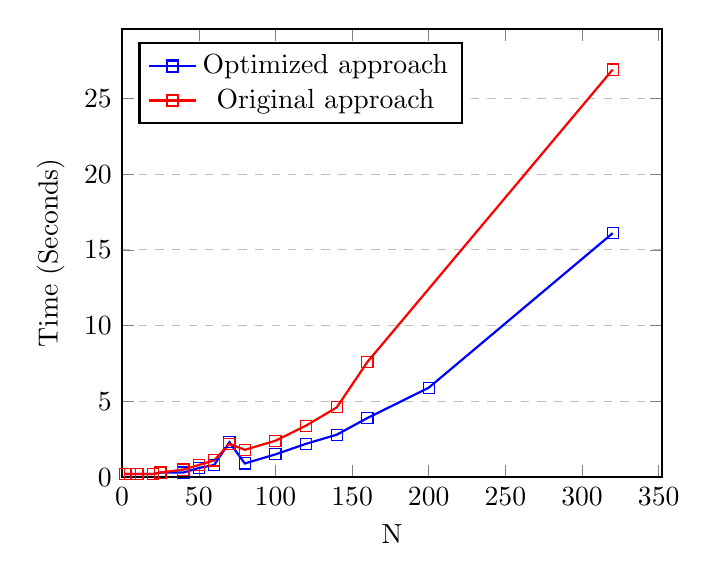
\begin{tikzpicture}
\begin{axis}[%legend pos=north west][
    %title={Time for finding a single solution for a N-Sequencer},
    xlabel={N},
    ylabel={Time (Seconds)},
    xmin=0, %xmax=160,
    ymin=0, %ymax=580,
   % xtick={0,2,5,10,20,40,50,60,80,100,120,160},
   % ytick={0,20,40,60,80,100,120},
    legend pos=north west,
    ymajorgrids=true,
    grid style=dashed
%    legend style={font=\fontsize{40}{50}\selectfont}, 
]
\addplot[
    color=blue,
    mark=square,
    ]
    coordinates {
    (2,0.2)(5,0.2)(10,0.2)(20,0.2)(25,0.3)(40,0.3)(50,0.6)(60,0.8)(70,2.3)(80,.9)(100,1.5)(120,2.2)(140,2.8)(160,3.9)(200,5.9)(320,16.1)
    };
    %\legend{Time for finding one  solution (seconds)}
      \addlegendentry{Optimized approach}
      \addplot[
    color=red,
    mark=square,
    ]
    coordinates {
    (2,0.2)(5,0.2)(10,0.2)(20,0.2)(25,0.3)(40,0.5)(50,0.8)(60,1.1)(70,2.2)(80,1.8)(100,2.4)(120,3.4)(140,4.6)(160,7.6)(320,26.9)
    };
%    \legend{Time for finding one  solution (seconds)}
  \addlegendentry{Original approach}
\end{axis}
\end{tikzpicture}
}
%%%%%%%%%%%%%%%%%%%%%%%%%%%%% 2
\centering
\subfloat[Size of the RCSP \label{ax:conssize}]{%
\pgfplotsset{width=6cm,compat=1.5}
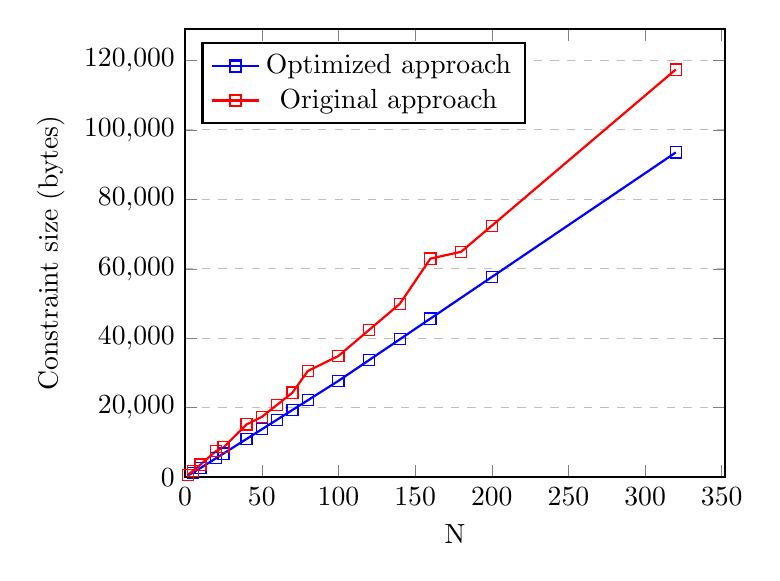
\begin{tikzpicture}
\begin{axis}[
   % title={Size of the RCSP constraints for a N-Sequencer},
    xlabel={N},
    ylabel={Constraint size (bytes)},
    xmin=0, %xmax=160,
    ymin=0, %ymax=100000,
   % xtick={0,2,5,10,20,40,50,60,80,100,120,160},
   % ytick={0,20,40,60,80,100,120},
    legend pos=north west,
    ymajorgrids=true,
    grid style=dashed,
   % legend style={font=\fontsize{40}{50}\selectfont},
    yticklabel style={/pgf/number format/fixed}, scaled ticks=false
]
 
\addplot[
    color=blue,
    mark=square,
    ]
    coordinates {
    (2,511)(5,1288)(10,2603)(20,5393)(25,6788)(40,10973)(50,13763)(60,16553)(70,19343)(80,22133)(100,27729)(120,33709)(140,39689)(160,45669)(200,57629)(320,93509)
    };
%    \legend{Approach2???}
  \addlegendentry{Optimized approach}

\addplot[
    color=red,
    mark=square,
    ]
    coordinates {
    (2,711)(5, 1788)(10,3609)(20,7459)(25,8552)(40,15159)(50,17327)(60,20837)(70,24347)(80,30559)(100,34901)(120,42401)(140,49901)(160,62945)(180,64901)(200,72401)(320,117401)
    };
    %\legend{Size of the RCSP constraints}
  \addlegendentry{Original approach}
\end{axis}
\end{tikzpicture}
}

%%%%%%%%%%%%%%%%%%%%%%%%%%%%% 3
\centering
\subfloat[Time (s), calculating the RLTS \label{ax:total}]{%
\pgfplotsset{width=6cm,compat=1.5}
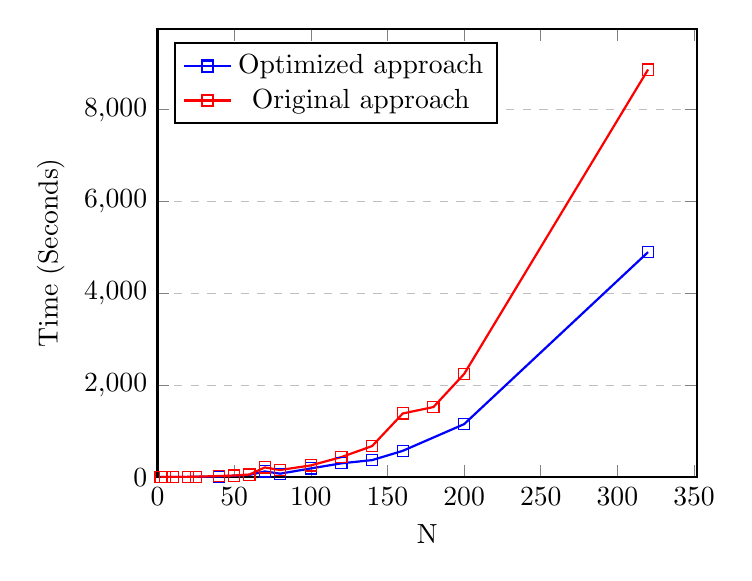
\begin{tikzpicture}
\begin{axis}[%legend pos=north west][
   % title={Calculating the RLTS of N-Sequencer},
    xlabel={N},
    ylabel={Time (Seconds)},
    xmin=0, %xmax=160,
    ymin=0, %ymax=580,
    %xtick={0,2,5,10,20,40,50,60,80,100,120,160},
   % ytick={0,20,40,60,80,100,120},
    legend pos=north west,
    ymajorgrids=true,
    grid style=dashed
 %   legend style={font=\fontsize{40}{50}\selectfont}, 
]
 
\addplot[
    color=blue,
    mark=square,
    ]
    coordinates {
    (2,0.4)(5,0.9)(10,1.8)(20,4.0)(25,7.9)(40,12.1)(50,29.1)(60,48.2)(70,122.8)(80,74.6)(100,188.4)(120,300.0)(140,369.7)(160,571.8)(200,1152.8)(320,4899.962)
    };
  %  \legend{Approach2???}
  \addlegendentry{Optimized approach}

\addplot[
    color=red,
    mark=square,
    ]
    coordinates {
    (2,0.4)(5, 1.1)(10,2.1)(20,5.2)(25,8.6)(40,22.4)(50,33.8)(60,55.7)(70,210.3)(80,154.5)(100,254.1)(120,436.2)(140,675.4)(160,1385.3)(180,1525.2)(200,2245.1)(320,8876.4)
    };
 %   \legend{Total time???}
   \addlegendentry{Original approach}
\end{axis}
\end{tikzpicture}
}
%%%%%%%%%%%%%%%%%%%%%%%%%%%%%%%%%%%%%%%%%%%%% 4
\centering
\subfloat[Time (s), building CA and connector coloring table \label{ax:caccsol}]{%
\pgfplotsset{width=6cm,compat=1.5}
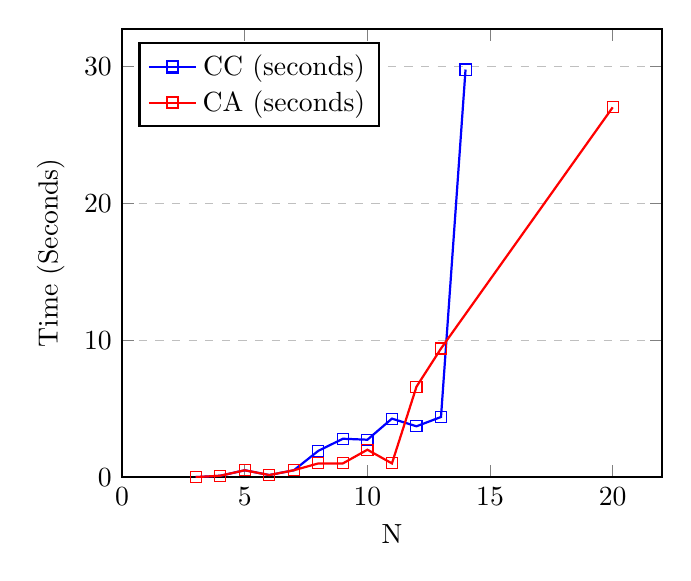
\begin{tikzpicture}
\begin{axis}[%legend pos=north west][
    %title={Time spent to calculate the coloring semantics of a N-Sequencer},
    xlabel={N},
    ylabel={Time (Seconds)},
    xmin=0, %xmax=160,
    ymin=0, %ymax=580,
   % xtick={0,2,5,10,20,40,50,60,80,100,120,160},
   % ytick={0,20,40,60,80,100,120},
    legend pos=north west,
    ymajorgrids=true,
    grid style=dashed,
%    legend style={font=\LARGE},
]
\addplot[
    color=blue,
    mark=square,
    ]
    coordinates {
    (3,0)(4,0.1)(5,0.5)(6,0.15)(7,0.5)(8,1.92)(9,2.8)(10,2.73)(11,4.27)(12,3.71)(13,4.39)(14,29.76)
    };
   \addlegendentry{CC (seconds)}
   \addplot[
    color=red,
    mark=square,
    ]
    coordinates {
    (3,0)(4,0.1)(5,0.5)(6,0.15)(7,0.5)(8,1)(9,1)(10,2)(11,1)(12,6.6)(13,9.39)(20,27)
    };
   \addlegendentry{CA (seconds)}
\end{axis}
\end{tikzpicture}
}
\caption{Performance evaluation based on N-Sequencer network}
\end{figure}

% \begin{figure}[t]
% \sub figure[Time for finding a single solution for a N-Sequencer]{
% \label{ax:onesol}
% \timetosinglesolution
% }
% \end{figure}
%%%%%%%%%%%%%%%%%%%%%%%%%%%%%%%%5
%%%%%%%%%%%%%%%%%%%%%%%%
\section{Conclusions}\label{sec:conclusions}%TODO % %VERY IMPORTANT:%Proofs of the algorithm correctness (it solves the issue - for a given Reo network/CASM, we obtain a proper CASM/ minimized CASM) and completeness (for any issue of the type the algorithm finds a solution - for any Reo network/CASM, an output will be generated) should be added!
%Right now nobody can see that your algorithm works, maybe this is just a random set of instructions...
In this chapter, we have presented a constraint-based framework that encodes the semantics of Reo networks as constraint satisfaction problems whose predicates are either Boolean propositions or numerical constraints. We presented a hybrid approach to find the solutions for these problems. 

An advantage of our approach is that it treats data constraints symbolically to mitigate the state explosion problem. From this solution, we construct the semantic model corresponding to a Reo network in the form of constraint automata with state memory. 

Our framework supports \emph{product} and \emph{hiding} operations on constraint automata. We have implemented and integrated our approach as a tool in the ECT. 
%In order to provide support for time-dependent behavior of a Reo connector, Timed Constraint Automata (TCA) can be included in our framework in a very similar way to Constraint Automata (CA). The time constraints can be encoded and solved as data constraints over variables defined for capturing time.
 In the next section, we use this framework to encode priority. It makes our work the most expressive framework that exists to analyze Reo networks. %Furthermore, we will prove soundness and completeness of the RCSP encoding of 
%To our knowledge, this is the first time symbolic data-aware 
